\documentclass[a4paper,12pt]{report}
\usepackage[latin1]{inputenc}
\usepackage[english]{babel}
\usepackage{graphicx} 
\usepackage{listings}
\usepackage{fancyvrb}
\usepackage{float}
% \usepackage{bera}% optional: just to have a nice mono-spaced font
\usepackage{xcolor}

\colorlet{punct}{red!60!black}
\definecolor{background}{HTML}{EEEEEE}
\definecolor{delim}{RGB}{20,105,176}
\colorlet{numb}{magenta!60!black}

\lstdefinelanguage{JSON}{
    basicstyle=\normalfont\ttfamily,
    numbers=left,
    numberstyle=\scriptsize,
    stepnumber=1,
    numbersep=8pt,
    showstringspaces=false,
    breaklines=true,
    frame=lines,
    backgroundcolor=\color{background},
    literate=
     *{0}{{{\color{numb}0}}}{1}
      {1}{{{\color{numb}1}}}{1}
      {2}{{{\color{numb}2}}}{1}
      {3}{{{\color{numb}3}}}{1}
      {4}{{{\color{numb}4}}}{1}
      {5}{{{\color{numb}5}}}{1}
      {6}{{{\color{numb}6}}}{1}
      {7}{{{\color{numb}7}}}{1}
      {8}{{{\color{numb}8}}}{1}
      {9}{{{\color{numb}9}}}{1}
      {:}{{{\color{punct}{:}}}}{1}
      {,}{{{\color{punct}{,}}}}{1}
      {\{}{{{\color{delim}{\{}}}}{1}
      {\}}{{{\color{delim}{\}}}}}{1}
      {[}{{{\color{delim}{[}}}}{1}
      {]}{{{\color{delim}{]}}}}{1},
}
\bibliographystyle{unsrt}
\begin{document}

\begin{titlepage}
\begin{center}

\includegraphics[width=5cm]{EURECOM_logo_quadri}
\\[3cm]
\textbf{\Huge{Managing Emails via a Smart Web Application}}
\\[1cm]
\textbf{\textsc{\LARGE{Semester Project Report}}}
\\[0.5cm]
\LARGE{Alessandro Artoni}
\\
\large{Spring 2013}
\\[8cm]
\columnsep3cm
\begin{tabular}{p{8cm} p{8.5cm}}
\small{\textbf{Supervisors:}\newline
Rapha\"el Troncy\newline
Giuseppe Rizzo} 
&
\small{\textbf{EURECOM\newline Multimedia Department}}
\end{tabular}
\end{center}
\end{titlepage}

 \tableofcontents

\chapter{Introduction}
Since its creation in 1993, email did not change much in the way we use it. Its basic idea is simple: a plain exchange of textual (HTML) messages through  the internet. Thanks to its simplicity today most of us receive a huge amount of emails in a single day which makes almost impossible to focus on what's important to us and leave for later what's secondary.

On the other end this huge amount of information is not exploited as we could: \emph{Entity Recognition}, \emph{Machine Learning} and \emph{Semantic Web} are only examples of the technologies that can be applied to take advantage of these giant datasets.

Along with extracting information from data comes the evolution of the web: from a collection of linked documents or \emph{Web Pages} to full fledged \emph{Web Applications}. Thanks to both the evolution of the development environment (HTML5, CSS3, ECMAScript 5) and the rise of mobile devices the web is fastly becoming the universal platform.

\section{Motivation for the project}

The need for a new approach to electronic mail is getting bigger and bigger along with the amount of messages we receive daily. Moreover we think the potential of building a clustering algorithm based on the entity recognition system provided by the NERD\footnote{http://nerd.eurecom.fr} (Named Entities Recognition and Disambiguation) framework developed in the Multimedia research group in Eurecom is very high and valuable for improving emails systems.


\chapter{Similar projects}

There is a lot of excitement about building and innovating the world of emails, both in universities and in IT companies. We studied some existing projects in order to understand what techniques have already been used, what are the major approaches used today and how we can build emails applications better.


These are the projects we studied in particular for mining data:
\begin{itemize}
\item Manu Aery and Sharma Chakravarthy developed eMailSift \cite{Aery2005}: an email classification system based on structure and content. They propose a supervised data mining technique based on the exploitation of the structure information present in email messages.
\item In \cite{Drezde2008} is described an approach to determine if a message should be ``replied to'' or if it ``requires attachments''. The focus is very specific but it is interesting to see that their approach used a global training set to try to make guess without a specific training set for each user. This idea lends us to think that clustering was to be preferred with respect to classification.
\item The CNR developed a system described in \cite{Manco2008} for \emph{Mining Categories for emails via clustering and pattern discovery}. It's based on a three step approach: k-means for clustering, FP-Growth to extract cluster description and a custom technique to update cluster description.
\end{itemize}

Considering the development of a Web Application as important as the clustering feature, we studied some of the commercial offer (or proposal) available on the market this day:
\begin{itemize}
\item GMail (\texttt{http://mail.google.com}) is by far the leader in the market and is considered to be the first \emph{AJAX} web app to be developed. While it offers some ``intelligent'' service (attachment prediction, ``important'' email labeling) it should be credited for building a great UI along with a reliable system.'
\item Alto Mail (\texttt{https://login.altomail.com/login/signin}) while still in closed beta and not available for the public (we didn't manage to try it out) aims to provide better understanding of email subscriptions: they state that Alto Mail understands that products like Facebook, Twitter, LinkedIn, Amazon, (and more?) regularly send notifications and receipts and make it easy to classify or group them. 
\item As a UI starting point we studied MyMail (\texttt{http://dennyshess.ch/mymail/}) which is a mocked up email web client. Its interface allows to manage a lot of different email folders at the same time, which is why we chose it.
\end{itemize}


\chapter{Architectural overview}
In the next chapters we are going to analyze the choice made while designing the system along with some technical description and specification about the implementation. This chapter is divided in three section which reflect the main parts of this project itself: the first part describes the overall architecture of the system, the second section details the implementation of the server-side part of the system together with the specifications of how the clustering algorithm works. In the last part we will describe the process of building the client side web application.

Although this document tries to separate as much as possible this three aspects we must point out that both the design and the development of the applications were much more parallel than sequential and so are some technical considerations regarding the overall architecture.

The application \emph{bettermail} is designed with this goal: to provide an intelligent system capable of extracting semantic information from the emails body and use them to automatically classify (label) emails. We investigate how a named entities based clustering approach could prove itself in make the email experience better by automating the email labeling process. Moreover the project aims to give the user a simple and intuitive user interface to access those information.
\begin{figure}[H]
  \centering
  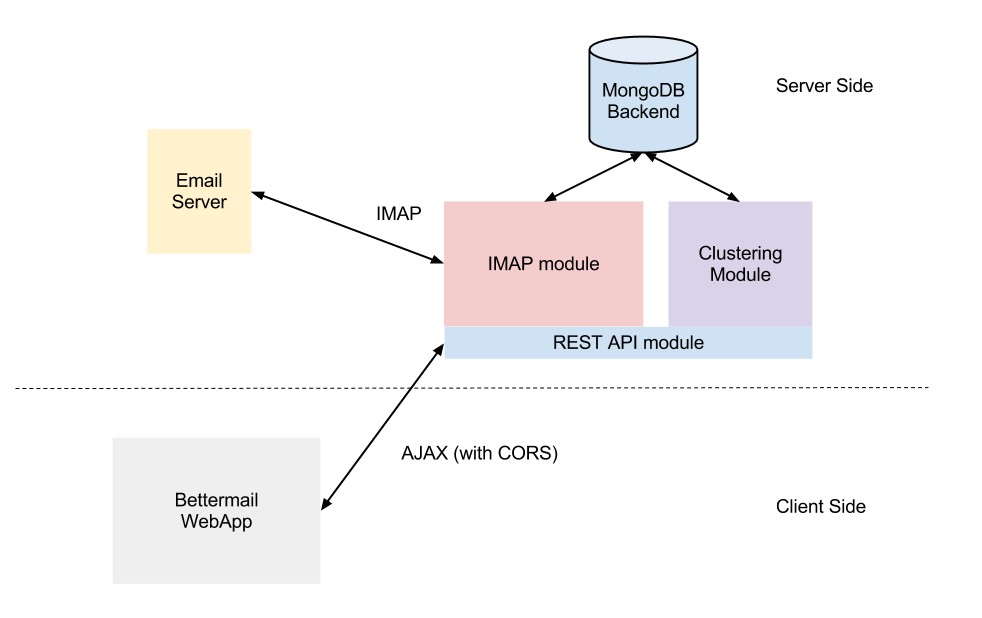
\includegraphics[width=15cm]{Architecture_Overview}
  \caption{The top level architecture of \emph{bettermail}}
  \label{fig:arch}
\end{figure}

As described in~\ref{fig:arch} the application is strongly separated in two parts: client and server side. Because the main idea is to build the client as a SPA\footnote{Single Page Application - http://en.wikipedia.org/wiki/Single-page\_application.} and at the same time to make the server functionalities available to potentially more then one client-side application we propose REST\footnote{Representational State Transfer - a style of software architecture for distributed system.} as the layer for building the main communication infrastructure. 
We first chose GMail as the targeted email service (mostly because of its wide diffusion) but the final choice was to use a generic IMAP connection to offer better integration with various email providers (although the application has been developed and tested with GMail).
\chapter{The Server}

The design and development of the server is one of the major activities of this project. Because our goal is to build a working application prototype from the ground up we first needed to get the integration with an existing email provider, thus we build the IMAP module. Next step was to expose this IMAP capabilities and, as discussed previously, we build a RESTfull web service to access it, which allow us to start working on the client too. After that we were finally able to start working on clustering and labeling.

\section{About general technical choices}
The whole server is built using Node.js. It is an event-driven system, built on top of Google's V8 javascript engine which provides a very fast and scalable infrastructure to build server side applications. Because of it's event-driven nature it has proved to be very suitable for I/O intensive application while being comparable to multi-threaded system under a CPU intensive workload. Among performances one of the main idea behind this choice is the developing paradigm. While building an application with a strongly typed language like Java requires a very long and precise designing phase to avoid the need of big refactoring, javascript is generally considered better for fast prototyping and Agile software development \footnote{Although the personal opinion of the authors is that javascript is a great language whatever the development model.}.

REST is chosen as the main API access point because of two main reasons: first of all it requires nothing but a client able to use basic HTTP verbs - in contrast with other system like SOAP that requires additional layers or WCF which is specific to a platform - and because it's generally simpler to reason about and define: once the resources' URI are defined the operations on them follows by the definition of RESTfull web service itself. 

All these services rely on a back-end database powered by MongoDB which is the natural choice for working in accordance with Agile development methodology and together with Node.js.

\section{Building the IMAP module}
The module responsible for handling the communication with the IMAP server has passed various iterations.
First we tried to build the basic functions to access the IMAP server: query for emails range, add and remove labels, retrieve email body, etc.\footnote{node-imap (https://github.com/mscdex/node-imap) and mailparser (https://github.com/andris9/mailparser.) had been used as a starting point.}. 

Subsequently, following the guidelines described in RFC4549\footnote{Synchronization Operations for Disconnected IMAP4 Client (http://www.faqs.org/rfcs/rfc4549.html).} we implemented a basic IMAP client (on the server) with support for incremental synchronization. 
All these features where then exposed via RESTfull APIs, described in the next chapter.

One of the major problems encountered within this phase resides in the sequential nature of the IMAP protocol itself. The first approach was to create a new connection with the IMAP server for each requested resource. While this approach seems fine when tested in a manual request sequence flow it turned out that GMail, like many other providers, impose a very low limit on the maximum number of concurrent requests for the same account (it is not specified in the documentation but we experienced it to be around 10). This behavior force us to a fixed, sequential approach, which solved the problem.

\section{The REST server}
For simplifying the process of building our APIs we decided to use \emph{express}, a Node.js framework.
Its architecture allows to define ``routes'' on which you can define the behavior for each separate HTTP verb. In addition, it provides a system for plug middleware in to intercept requests before routes handler(for example authenticating user before serving the request). We used this feature to implement a CORS\footnote{Cross-origin resource sharing, a new standard to allow web applications to safely bypass the same origin policy.} compliant web service.

These are the main resources defined with the associated URI.Except for labels, the service supports the GET verb only because the first goal of the application is email reading and retrieving. Anyway the architecture would allow to easily add feature like deleting or sending new emails provided to use an SMTP module which at the moment we didn't yet wrote.
Each method exchanges information in the JSON format. The structure of the returned item is listed after each resource.
\begin{itemize}
\item \texttt{/boxes}: The list of all the mailbox available.
\begin{lstlisting}[language=JSON]
[
  {
    "attribs": [
      "HASNOCHILDREN"
    ],
    "delimiter": "/",
    "name": "SomeLabelName"
  },
  //...
]
\end{lstlisting}
\item \texttt{/boxes/:boxId}: The details of the mailbox specified by the boxId
\begin{lstlisting}[language=JSON]
{
  "uidnext": 293,
  "readOnly": true,
  "flags": [
    "Answered",
    "Flagged",
    "Draft",
    //...
  ],
  "newKeywords": false,
  "uidvalidity": 30,
  "keywords": [
    ""
  ],
  "permFlags": [],
  "name": "SomeLabelName",
  "messages": {
    "total": 279,
    "new": 0
  }
}
\end{lstlisting}
\item \texttt{/boxes/:boxId/:mailUid}: The full body of the specified email (identified by \texttt{boxId} AND \texttt{mailUid})
\begin{lstlisting}[language=JSON]
{
  "text": "someText",
  "html": "<html>someHtml</html>",
  "headers": {
    "delivered-to": "artoale@gmail.com",
    "received": [...]
    //...
  },
  "subject": "aSubject",
  "references": [
    // Related email messageId
  ],
  "messageId": "aMessageId",
  "inReplyTo": [
    "anotherMsgId"
  ],
  "priority": "normal",
  "from": [
    {
      "address": "someOne@gmail.com",
      "name": "Some One"
    }
  ],
  "to": [
    {
      "address": "me@gmail.com",
      "name": "Alessandro Artoni"
    }
  ],
  "seqno": 146,
  "uid": 153,
  "flags": [
    "\\Seen"
  ],
  "date": "24-Oct-2010 18:10:53 +0000",
  "_events": {},
  "x-gm-thrid": "1350194035284457856",
  "x-gm-msgid": "1350507014051968106",
  "x-gm-labels": [
    "\\\\Inbox",
    "\\\\Important"
  ]
}
\end{lstlisting}
\item \texttt{/boxes/:boxId/unseen}: The headers and mime structure of  all the unseen emails in the specified mailbox
\begin{lstlisting}[language=JSON]
[
  {
    //an object like the previous example but without text and HTML 
  },
  //more objects...
]
\end{lstlisting}
\item \texttt{/boxes/:boxId/:mailUid/labels}: The list of labels assigned to the specified email
\begin{lstlisting}[language=JSON]
[
  "\\\\Inbox",
  "\\\\Important",
  //...
]
\end{lstlisting}
\item \texttt{/boxes/:boxId/from/:startUid}: The structure and headers of all emails in a specific mailbox with an UID strictly bigger than \texttt{startUid}.
\item \texttt{/boxes/:boxId/from/:startUid/to/:endUid}: The structure and headers of all emails in a specific mailbox with an UID ranging from \texttt{startUid} (excluded) to \texttt{endUid}(included). If \texttt{endUid} is bigger then the maximum UID available this URI is equivalent to the previous one.
\item \texttt{/sync/:boxId}: Start a new synchronization of the specified mailbox. This URI fires the synchronization mechanism described in the previous section.
\end{itemize}

\section{Named Entity Recognition}
Each email content is first parsed by the NERD framework thanks to the node module provided by the team\footnote{https://github.com/giusepperizzo/nerd4node.}. The email body is then annotated with a set of information; for our work we considered two of them: \texttt{NerdType} which represents the ``high level'' class of the part of the text considered (e.g. Person, Thing, Date ...) and \texttt{label}, the specific entity recognized by NERD (e.g. Barack Obama, Personal Computer,the year 2012 ...). 
Those information are then stored permanently on the database for subsequent elaboration.

\section{The clustering algorithm}
The basic machine learning algorithm to labeling emails is divided in two step: starting centroids definition and clustering. This technique is inspired by that described by \cite{Manco2008} but it tries to exploit as much as possible the structured information from the email.



\subsection{Defining Centroids}
Instead of using a pure k-means approach with random starting centroids we choose to first use an Agglomerative Hybrid Clustering (AHC) implementation on a randomly selected subsets of emails. This algorithm outputs a tree known as a \emph{dendogram} in which each node corresponds to a partition of the clusters and its children to progressive sub-partitions. We traverse this three selecting all the node smaller then a parameter $L$ as basic clusters.
For each of this base clusters (if they're bigger than $L/k$ with $k$ parameter) we pick a random element in it as one of the starting centroids for the next step.

\subsection{K-Means}
The last step in the clustering algorithm is to apply a slightly modified version of k-means with \emph{linkage} criterion. As described above: instead of starting from randomly selected centroids we tried to exploit some knowledge to improve the clusters quality. While the AHC was executed on a subset of emails for performance reasons, we run k-means over the whole dataset.

\subsection{Metrics}
We gradually added features ($F_{i}$) to the definitions of our distance functions (one for each step):
\begin{itemize}
\item $F_{1}$: NERD type extracted (only if text field available, no HTML)
\item $F_{2}$: Email address (in both \emph{from} and \emph{to} fields)
\item $F_{3}$: Datetime 
\item $F_{4}$: Named entity label
\end{itemize}

This features are then used to computed a coefficient $C_{i}$, one per feature, with this relationship:
\[C_{i} = F_{i}^3 / 3 \]
Each coefficient is then normalized and multiplied by a wheight $w_{i}$, depending on the clustering technique used as follow:
\[distance = 1 - \sum_{i=1}^{4} g(C_i)*w_i \]
where $g$ is a function for normalizing values between 0 and 1 and $w$ is $[0.7, 0, 0, 0.3]$ for AHC and $[0.4, 0, 0.1, 0.5]$ for k-means.
\chapter{Building the client}
Multiple approaches on which type of client to develop are available. Among other ideas the two main possible approaches we considered are:
\begin{itemize}
\item adding features to an existing web client (GMail, Hotmail, etc...) by using either public APIs provided or by hacking the basic website by introducing script with browser extensions (Greasemonkey, Tampermonkey, ...)
\item creating a basic email web client from scratch
\end{itemize}

Because the first approach seems more reasonable in terms of time and efforts we picked it as first choice, specifically targeting GMail. After few tries with prototyping and reading a lot of documentation\footnote{https://developers.google.com/gadgets/} two problems arose: first of all the main APIs for adding functionalities to gmail is deprecated and won't be supported after July 2013. On the other end as the term itself suggests, hacking the website is full of problems: programming it's tedious, it requires a lot of DOM manipulation and traversing, done without a clear specification of how the HTML is structured and thus, how to manipulate it and there is no guarantee for the page structure not to change without notice.

For this reasons our final solution is a basic, web based, email client.
\section{Design}

The design proposed for the application follows three main principles: it should be simple, effective and (possibly) good looking.
While most of the web applications in the wild use a similar approach for organizing emails labels or folders, we think that a different design concept could strongly improve both the usability and the simplicity.

The common approach nowadays is to have a big list of emails - the current folder - and some sort of sidebar or navigation menu for switching between folders. 
We believe that in a scenario where the user make intense use of classification tool for dividing his email this design is suboptimal.
One main drawback have been identified: there is no easy way to have an overview of your folders.
This considerations leads to the solution we propose.

\subsection{Sketches}

\subsubsection{Design Concept: a GMail plug-in}
\begin{figure}[H]
  \centering
  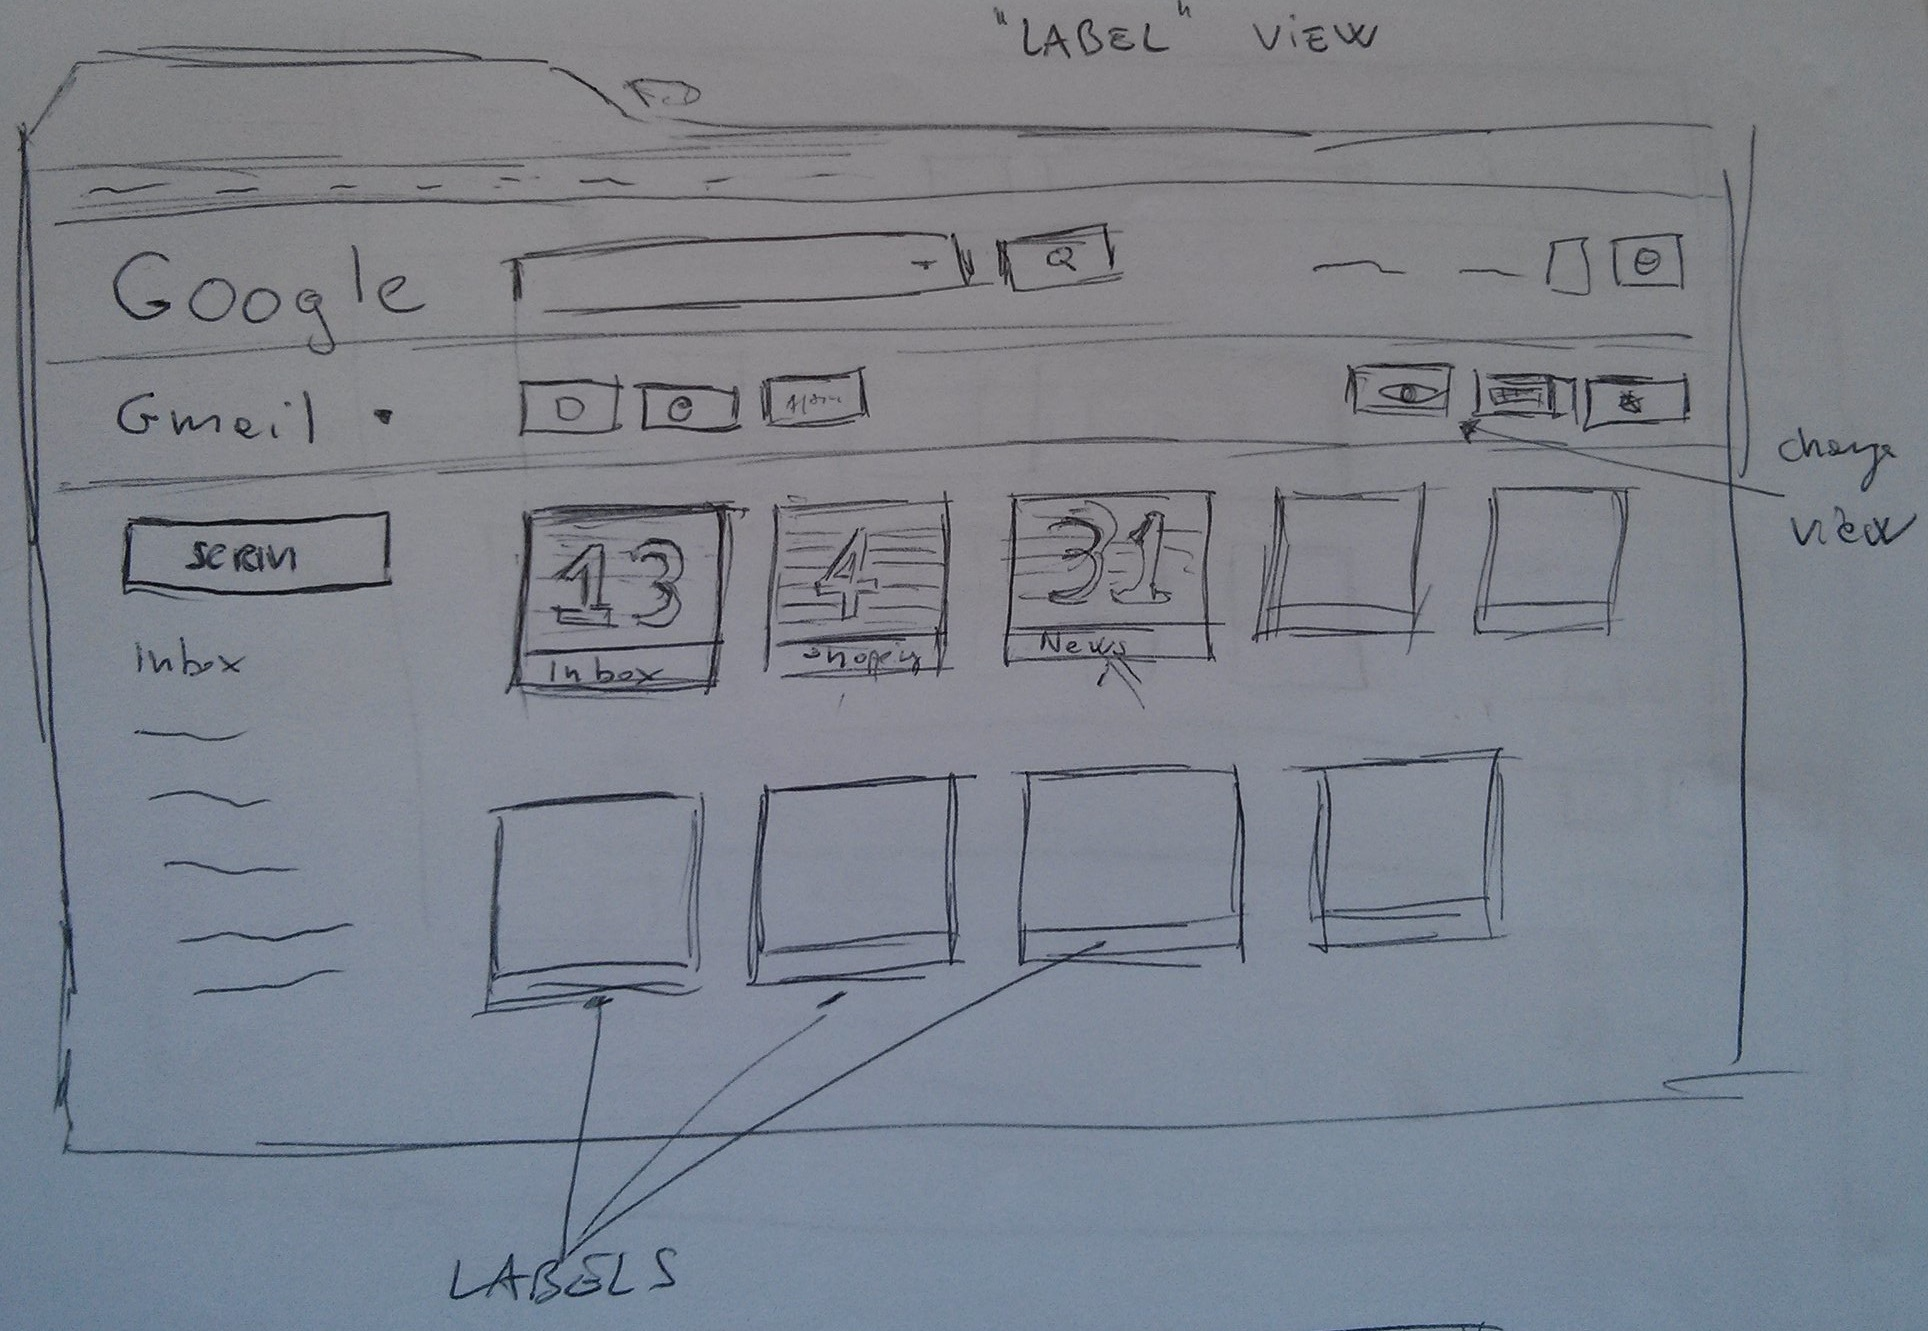
\includegraphics[height=1.5in]{old_grid}
  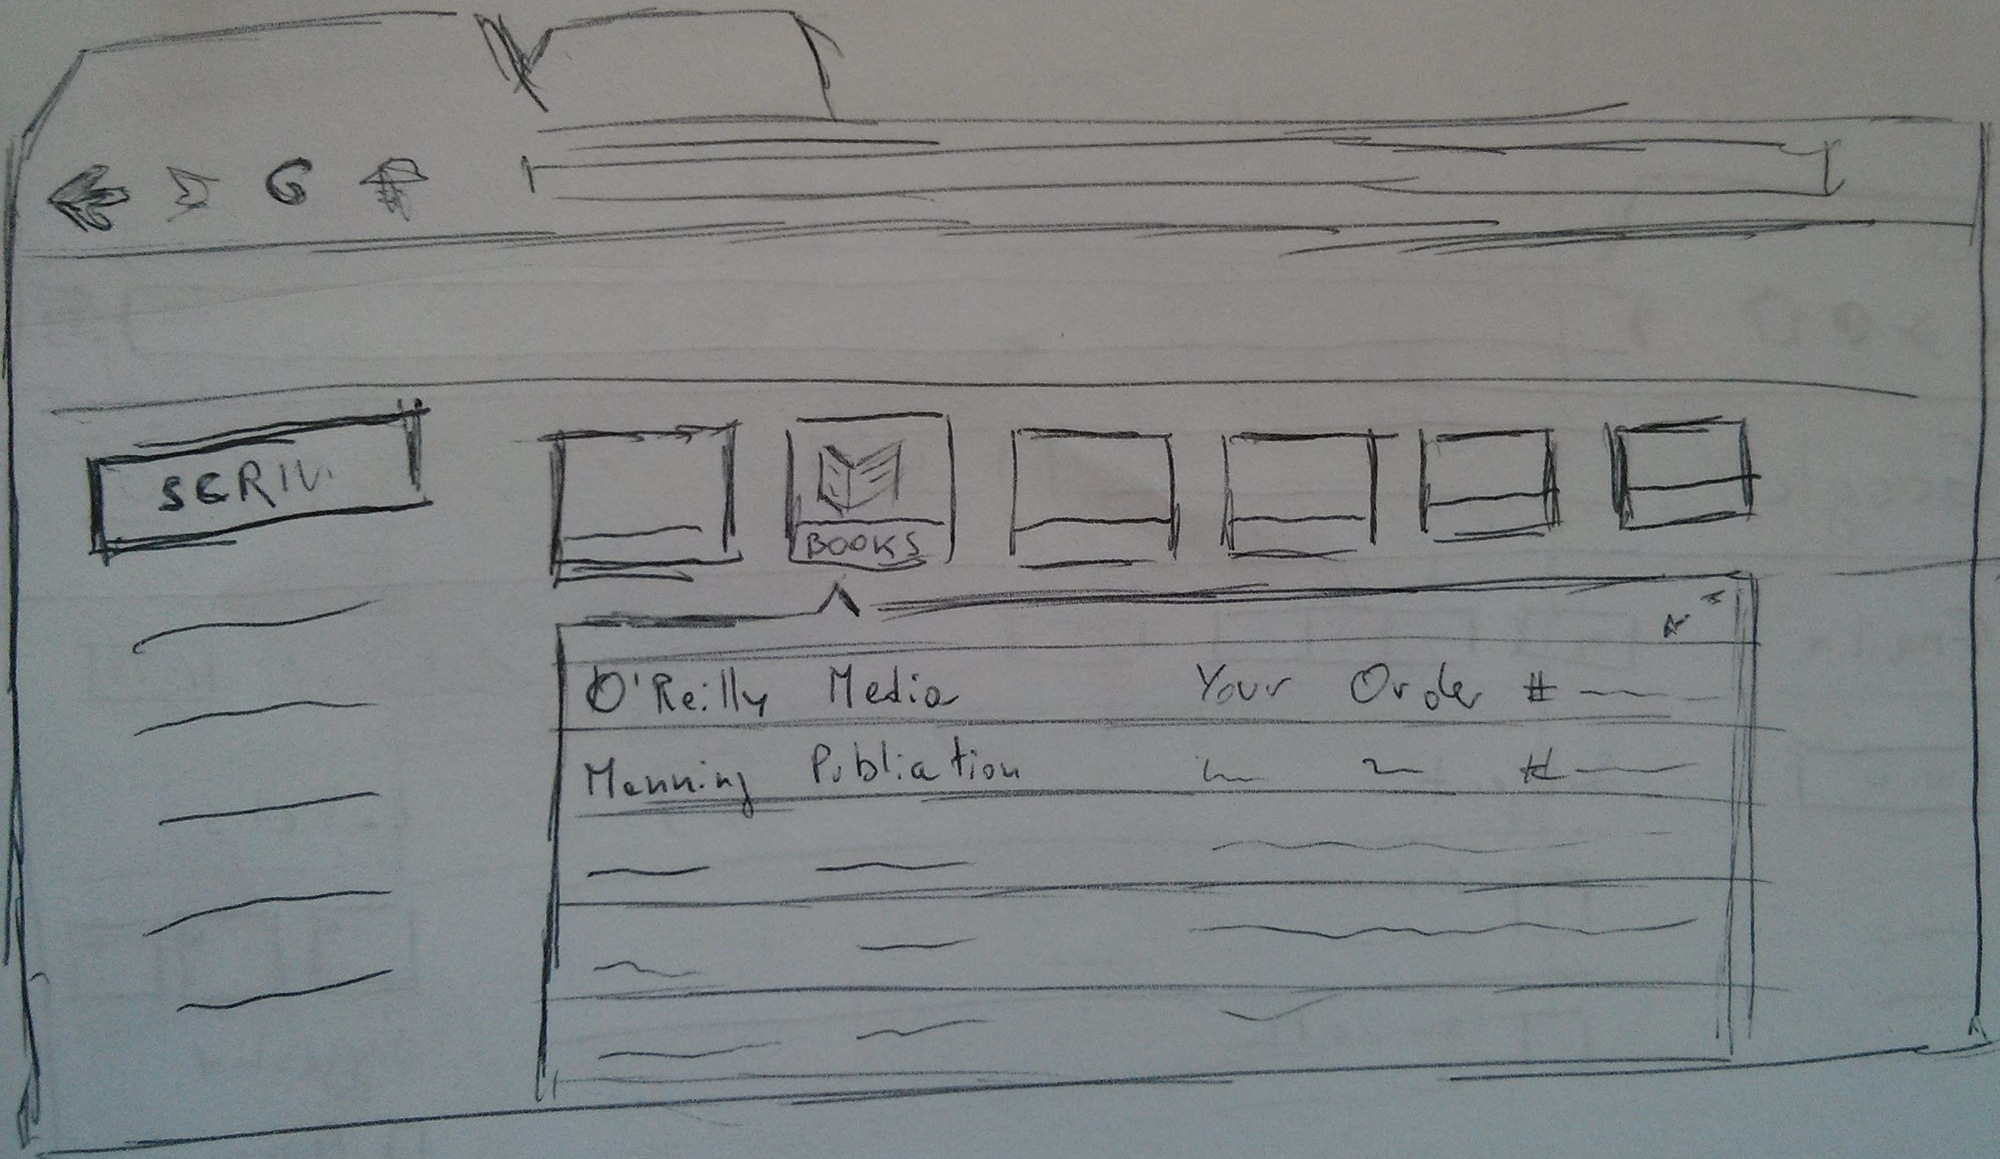
\includegraphics[height=1.5in]{old_grid_open}
  \caption{The first design idea concept grid view}
  \label{fig:old1}
\end{figure}
Figure~\ref{fig:old1} shows the first application concept: the main GMail list is replaced by a grid system, with one cell for each label. Each box contains basic information on the mailbox like the number of unread messages over the total, last message date and so on.
When a box is clicked it shows the classic GMail emails list with the option to expand and pass to normal label view. 

\begin{figure}[H]
  \centering
  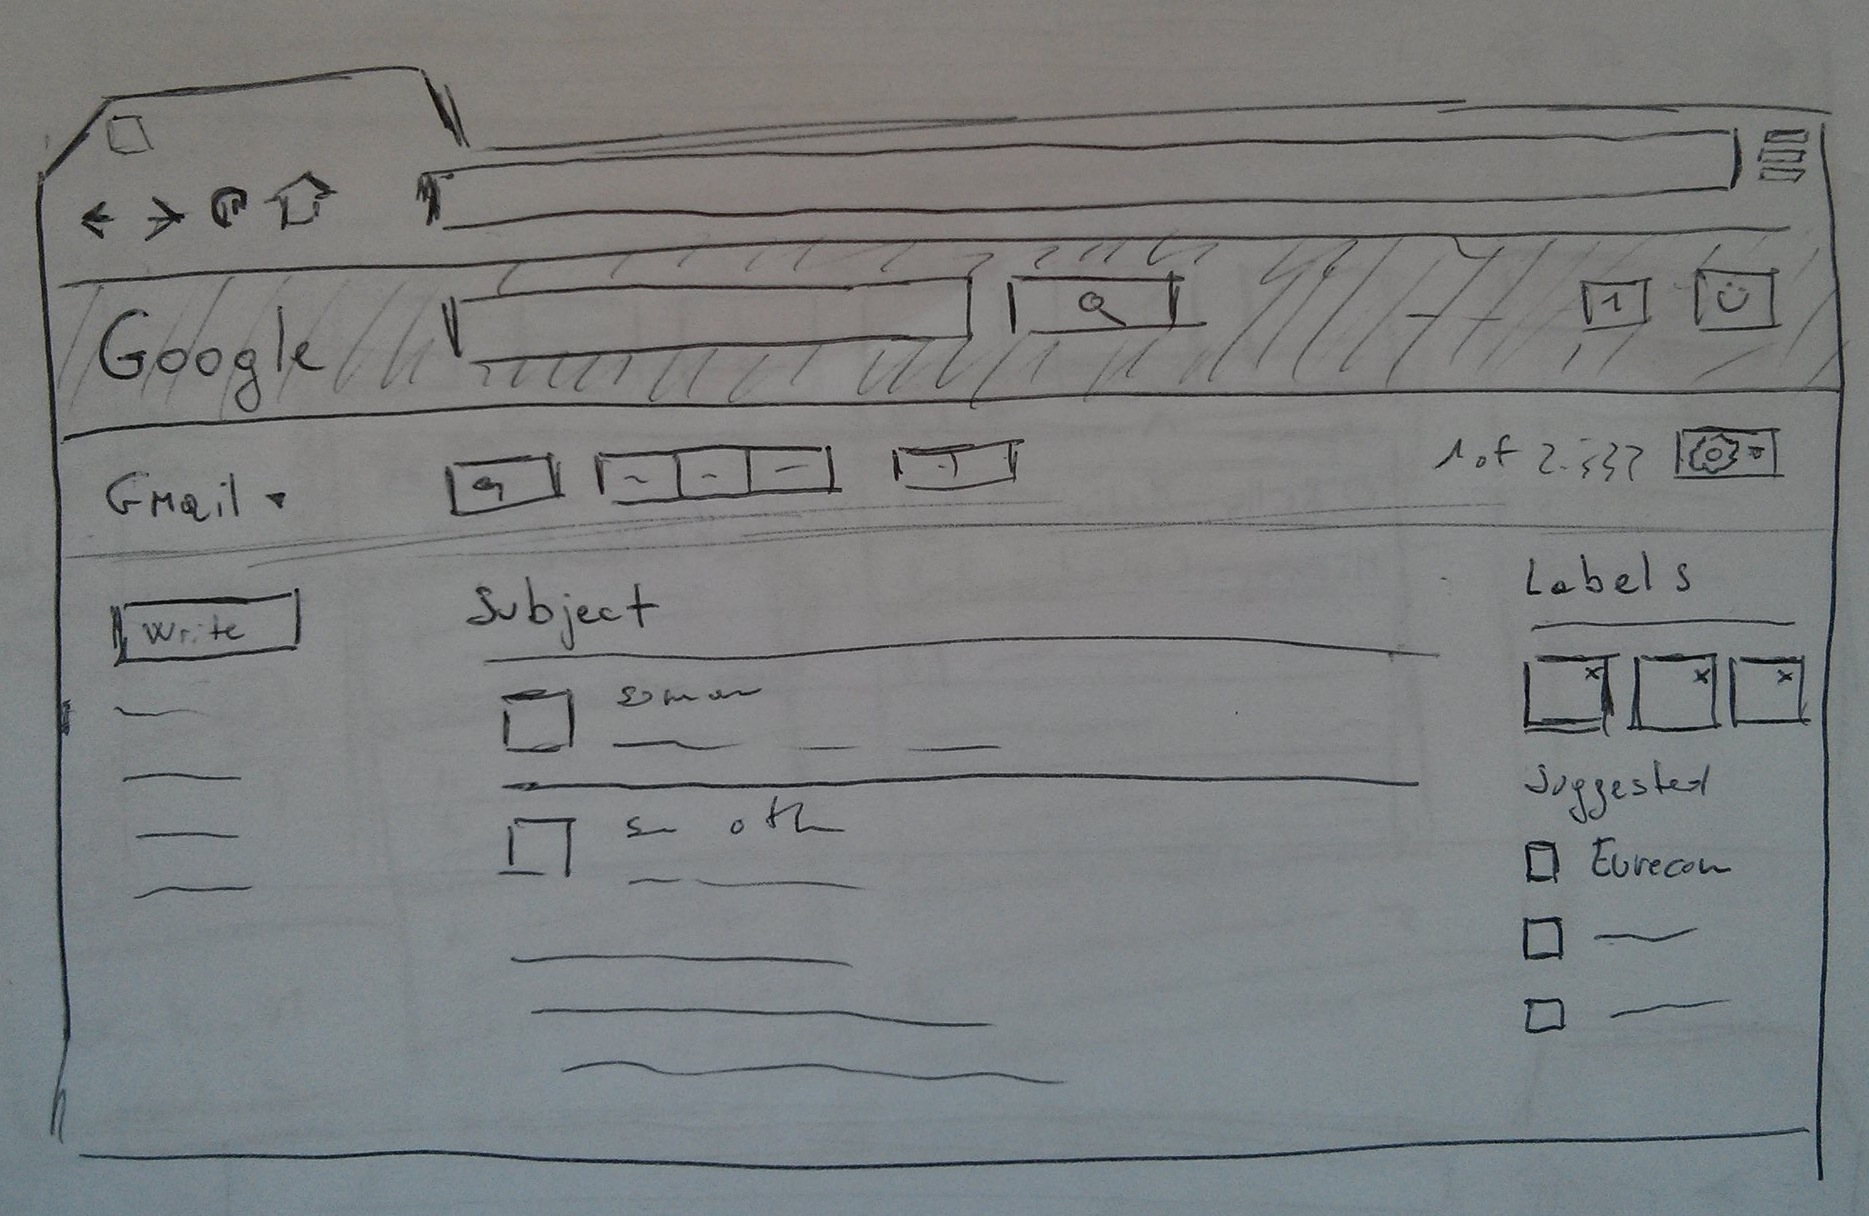
\includegraphics[height=2in]{old_label}
  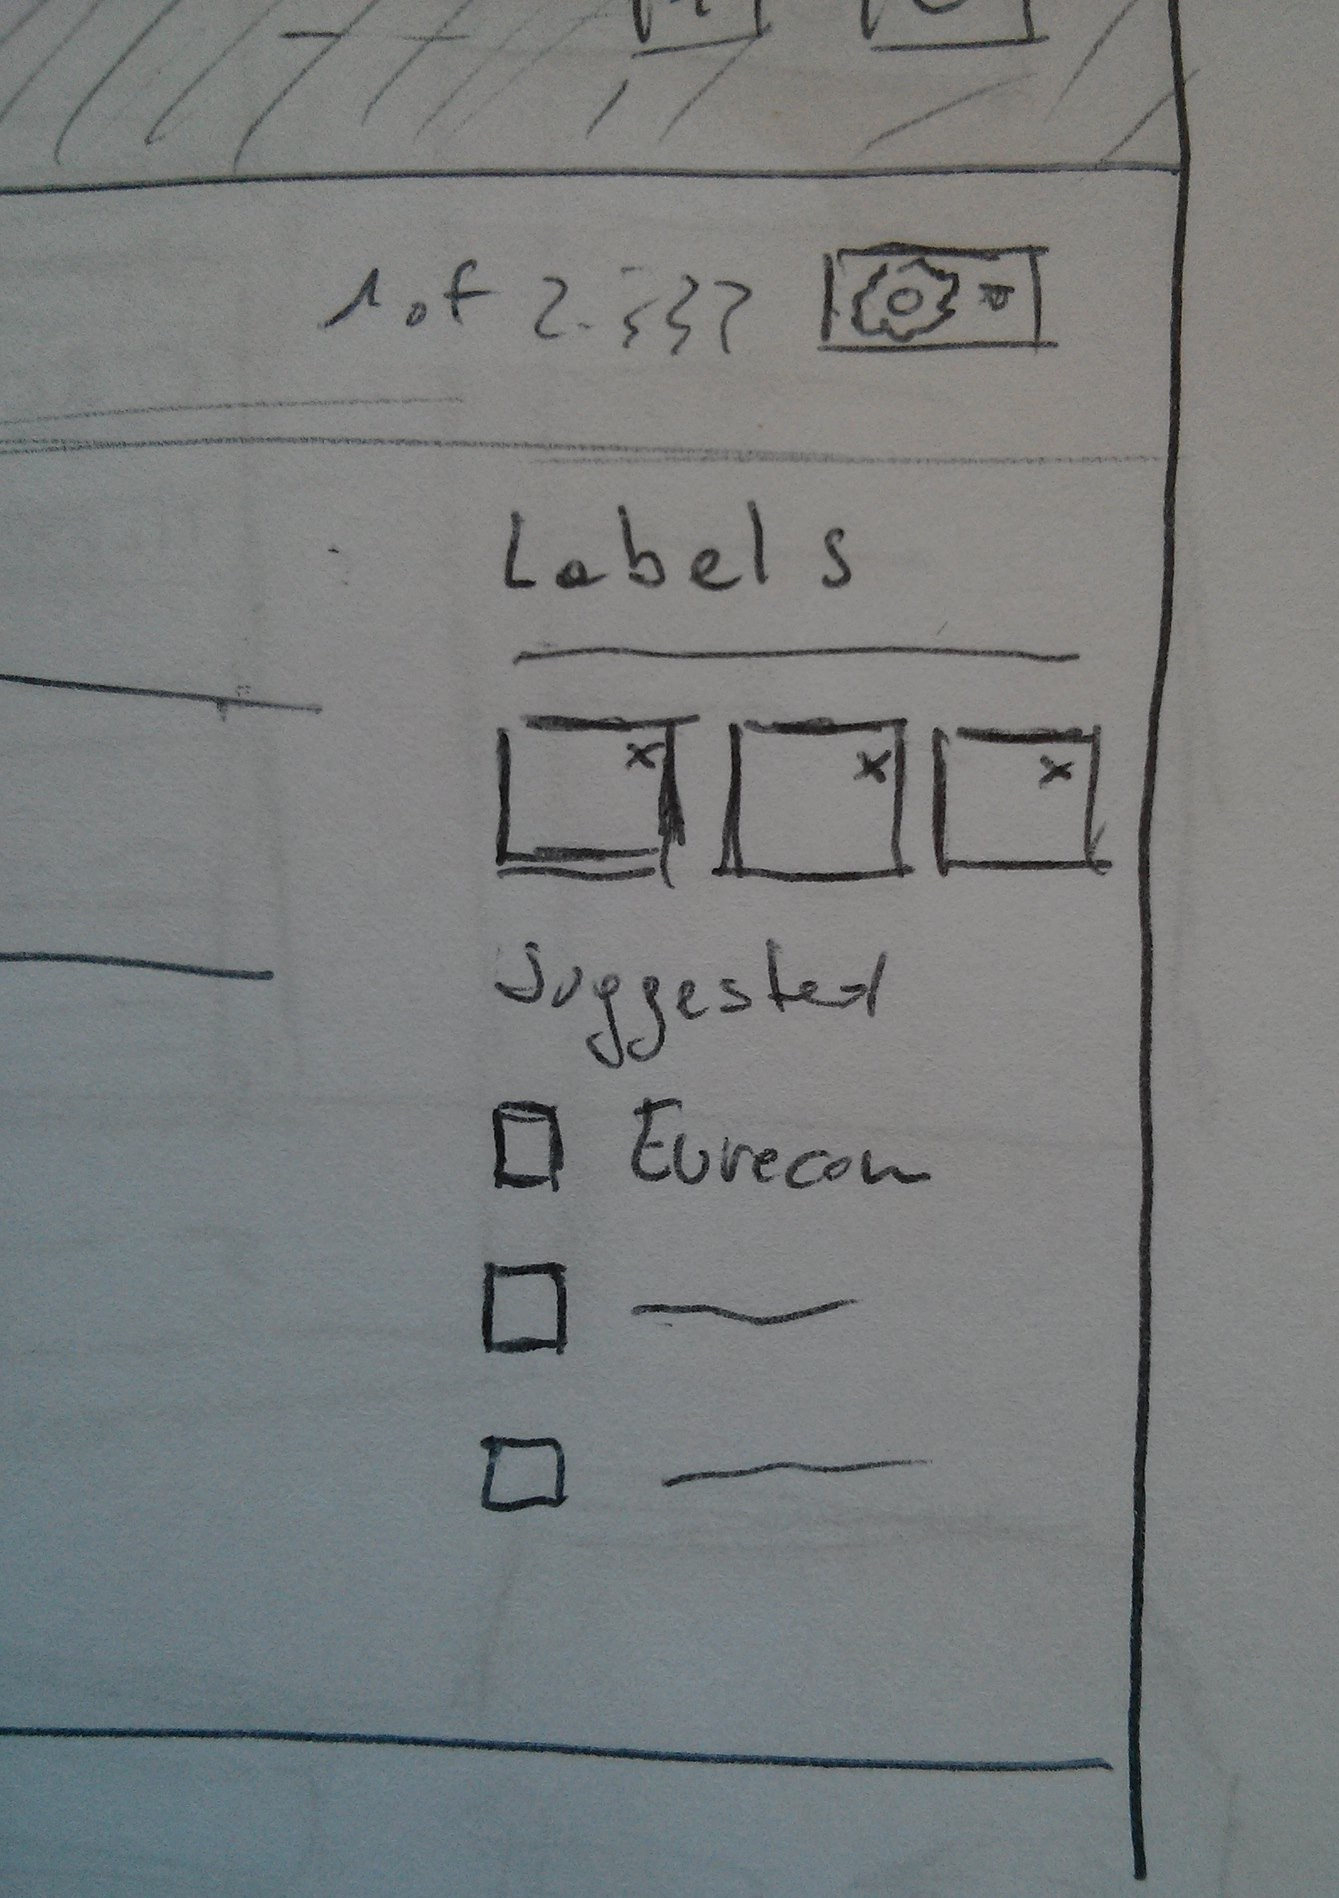
\includegraphics[height=2in]{old_label_detail}
  \caption{How to add labeling information to GMail}
  \label{fig:old2}
\end{figure}
In~\ref{fig:old2} is shown the basic idea of how to intensify labeling features in Google mail interface. Because there is no much space available in the page, we tried to exploit the blank one on the right, which is rather small but the only one available. It shows a small box, one for each label assigned to the email and a list of suggested labels, which were supposed to be extracted by the ``intelligent'' module of the system.

Because the GMail plug-in solution turned out to be unfeasible, we had to discard it (while the basic grid system was already implemented as an AngularJS directive\footnote{This directive is available at https://github.com/artoale/griddy.}) as shown in ~\ref{fig:griddy}.
\begin{figure}[H]
  \centering
  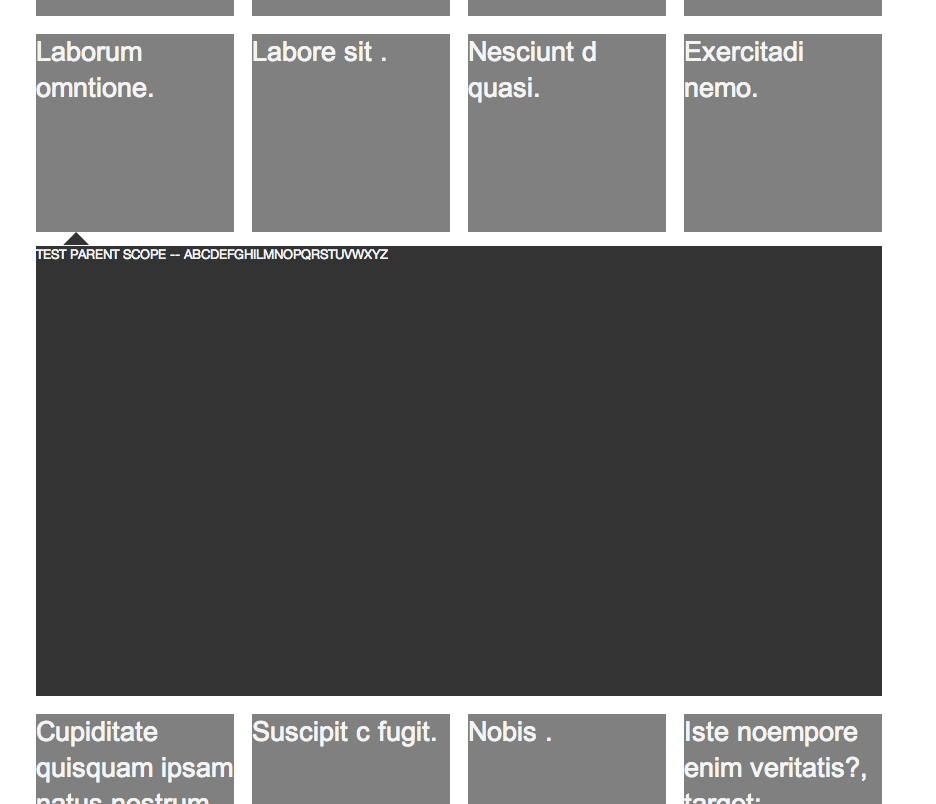
\includegraphics[width=4in]{griddy}
  \caption{Griddy directive prototype}
  \label{fig:griddy}
\end{figure}
\subsubsection{Next level: a new web mail}

\begin{figure}[H]
  \centering
  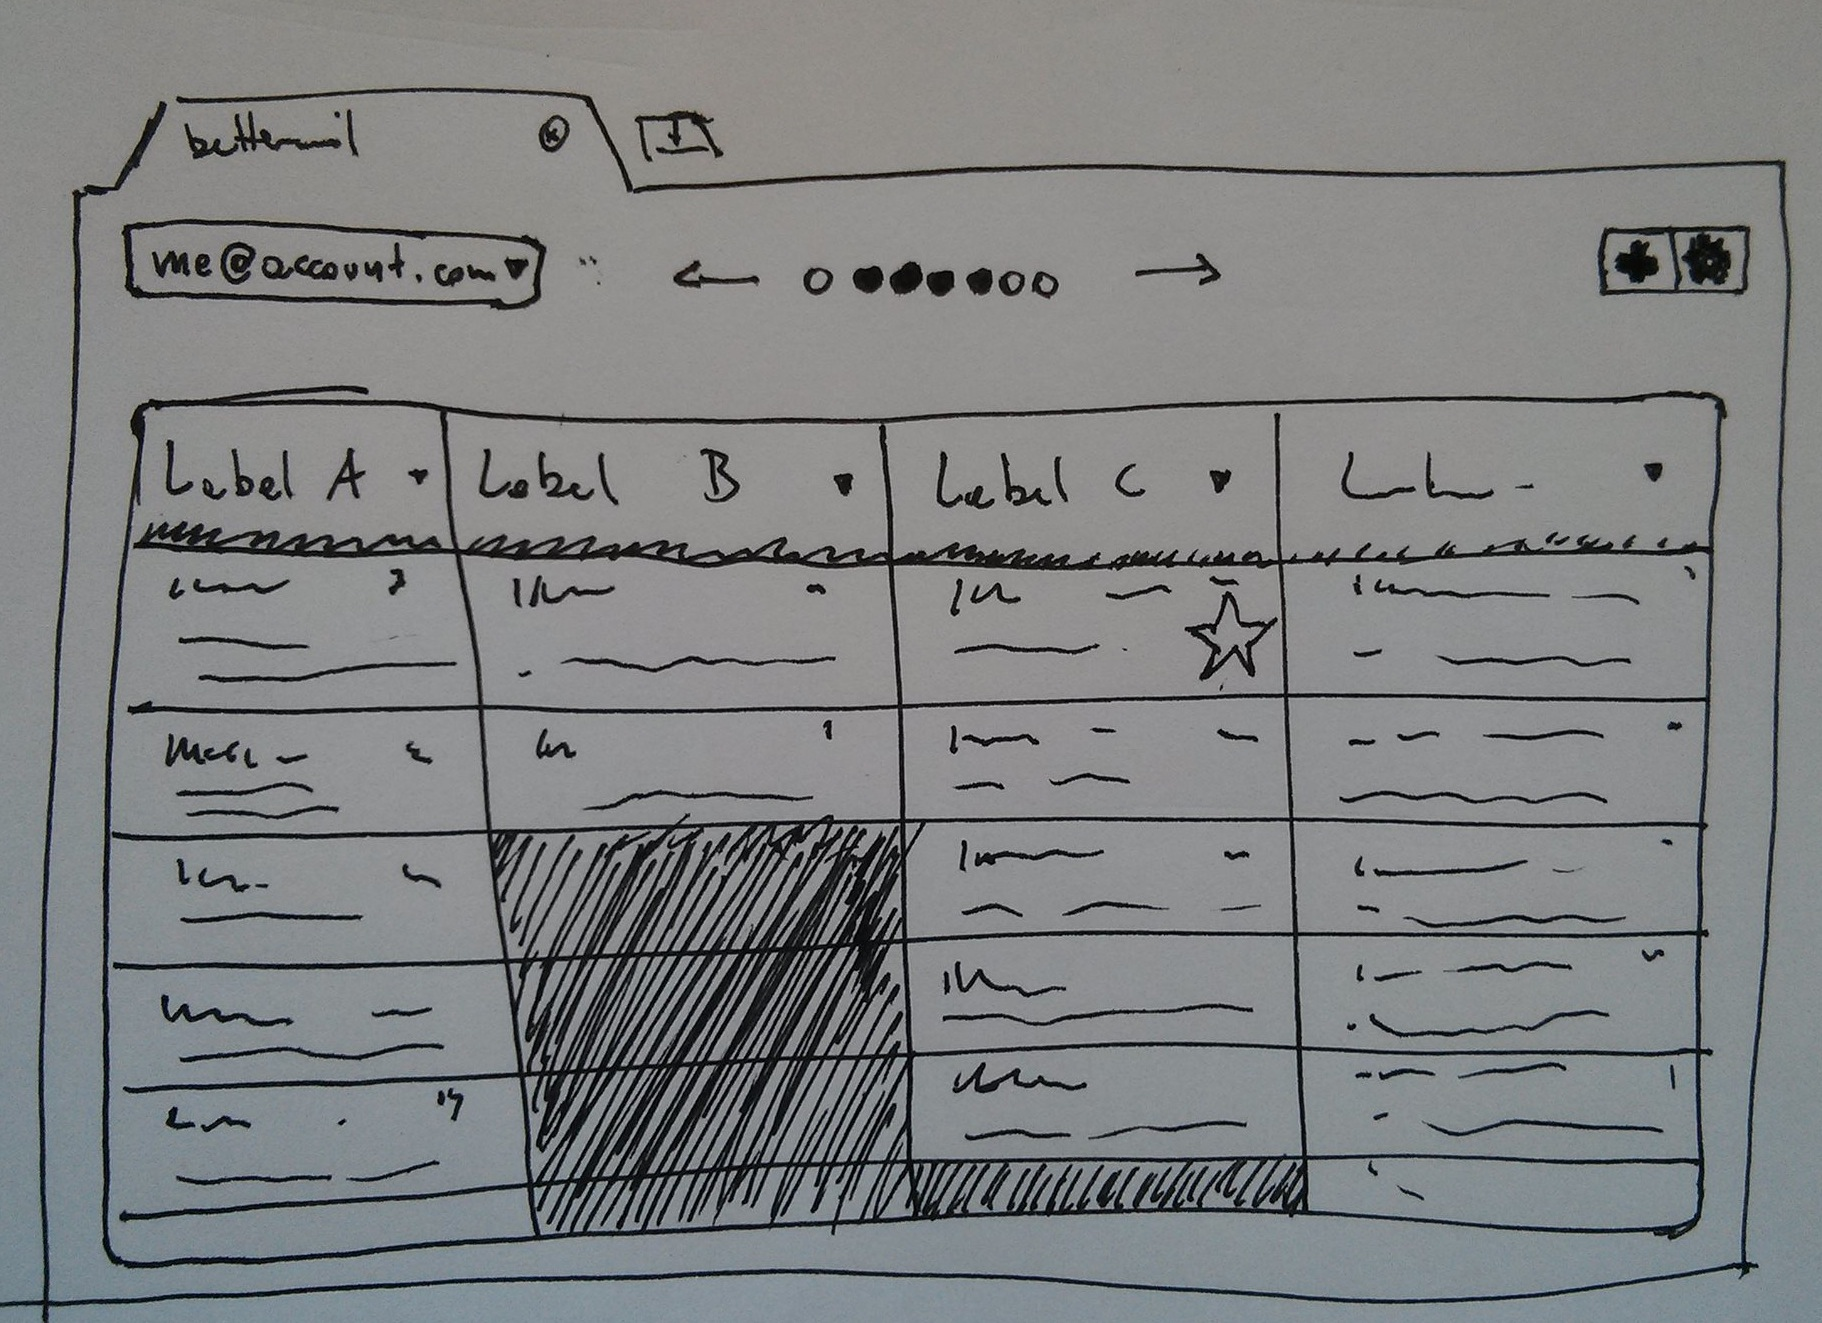
\includegraphics[width=4in]{new}
  \caption{Sketch of \emph{bettermail} main interface}
  \label{fig:new1}
\end{figure}
As you can see from figure~\ref{fig:new1} we propose a novel design based on a column system. 
Each column contains email from a specific label, with summary information (sender, date and time, starred flag, first email words). The number of column showed is supposed to be adaptable depending on the screen size. 


\begin{figure}[H]
  \centering
  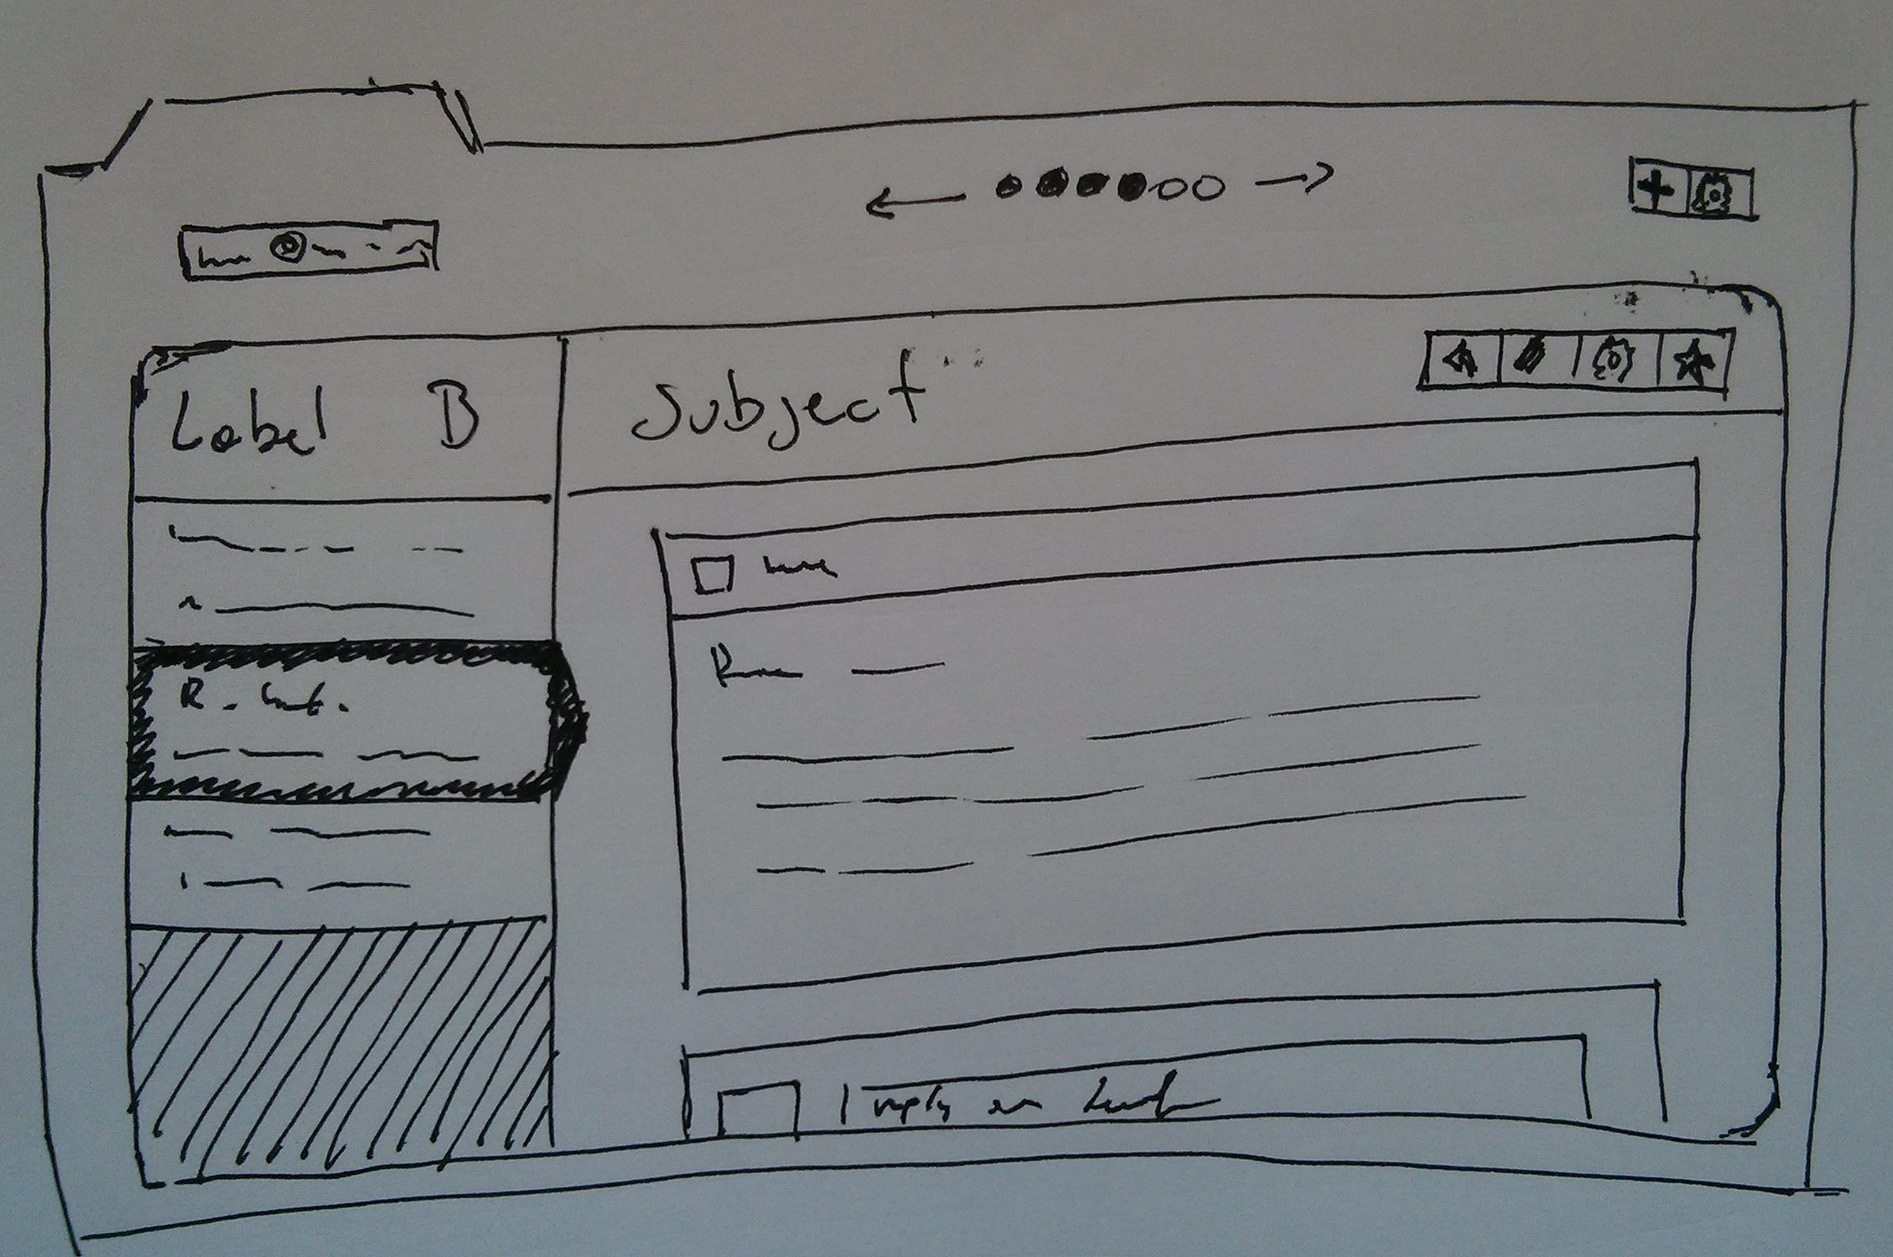
\includegraphics[width=4in]{new_2_cols}
  \caption{Detail of an open email}
  \label{fig:new2}
\end{figure}

When a specific email is selected the relative column is moved to the left, the email highlighted and the content is shown on the right, replacing the other columns (~\ref{fig:new2}).

\begin{figure}[H]
  \centering
  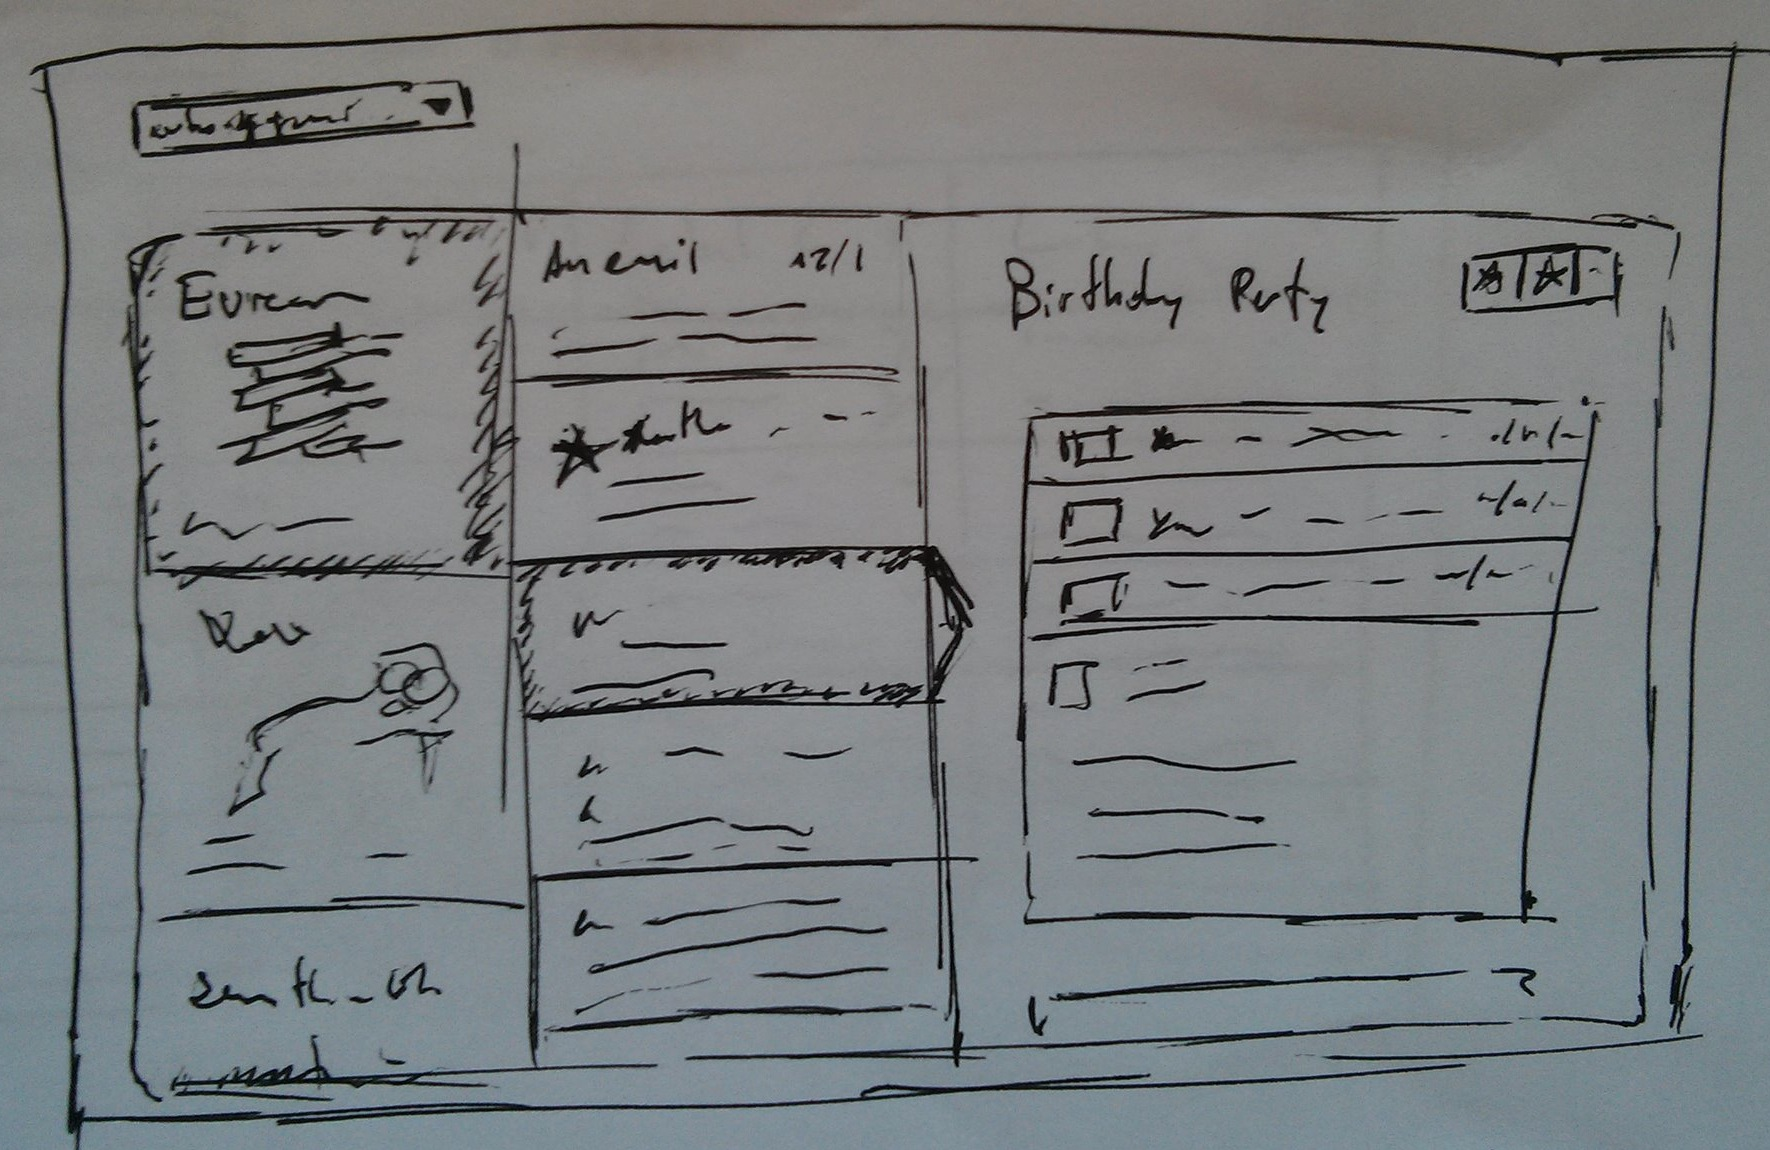
\includegraphics[width=4in]{new_3_cols}
  \caption{An additional view for users with many folders}
  \label{fig:new3}
\end{figure}
An additional view we designed is here reported in~\ref{fig:new3}(even if not implemented) for user with a large number of labels/folders for whom the number of columns may be a limit. In this case each column contains a box (much like the proposed GMail grid) which is expandable in the message list which behave like the basic homepage.

\subsubsection{Thinking mobile}
Because of the growth of the smartphone market it is considered good practice to develop web application thinking mobile first, in order to allow for all the features to be present in the application whatever the screen resolution or size. We propose in figure~\ref{fig:mobile} the ``natural'' adaptation of the desktop application to the mobile world, where a single column is displayed on screen and moving between column is a swipe gesture.
\begin{figure}[H]
  \centering
  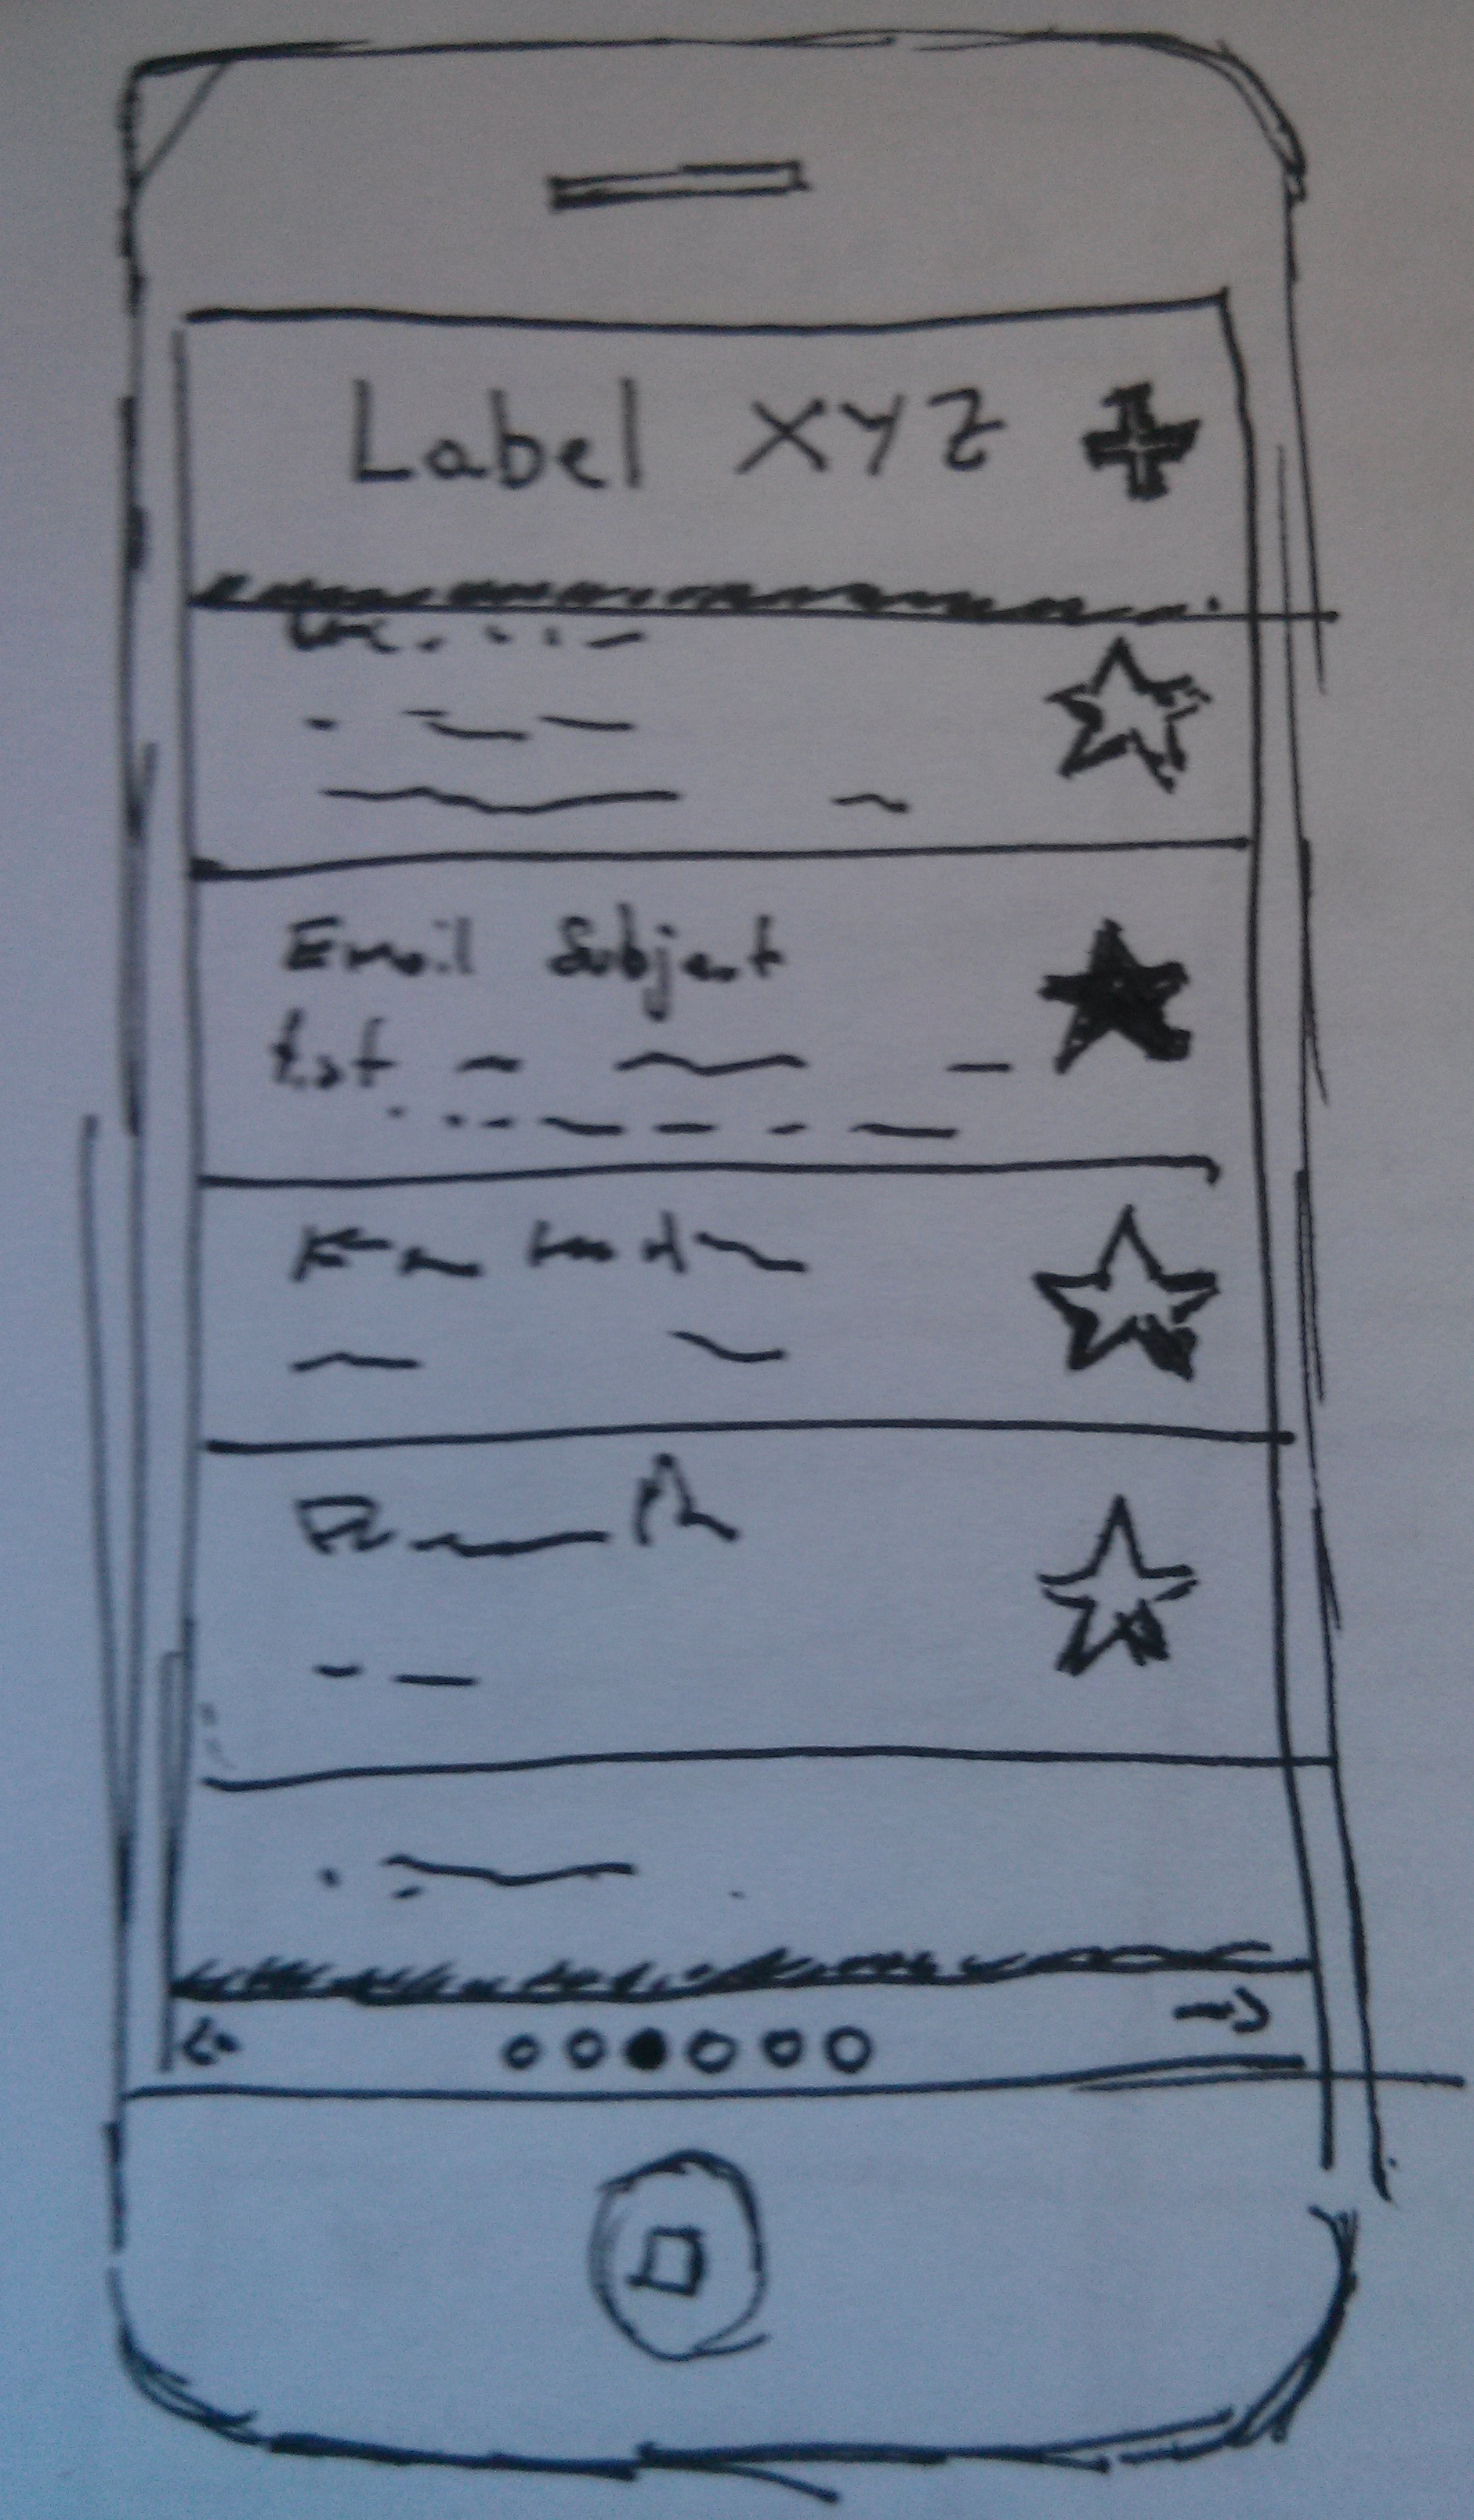
\includegraphics[height=2in]{list}
  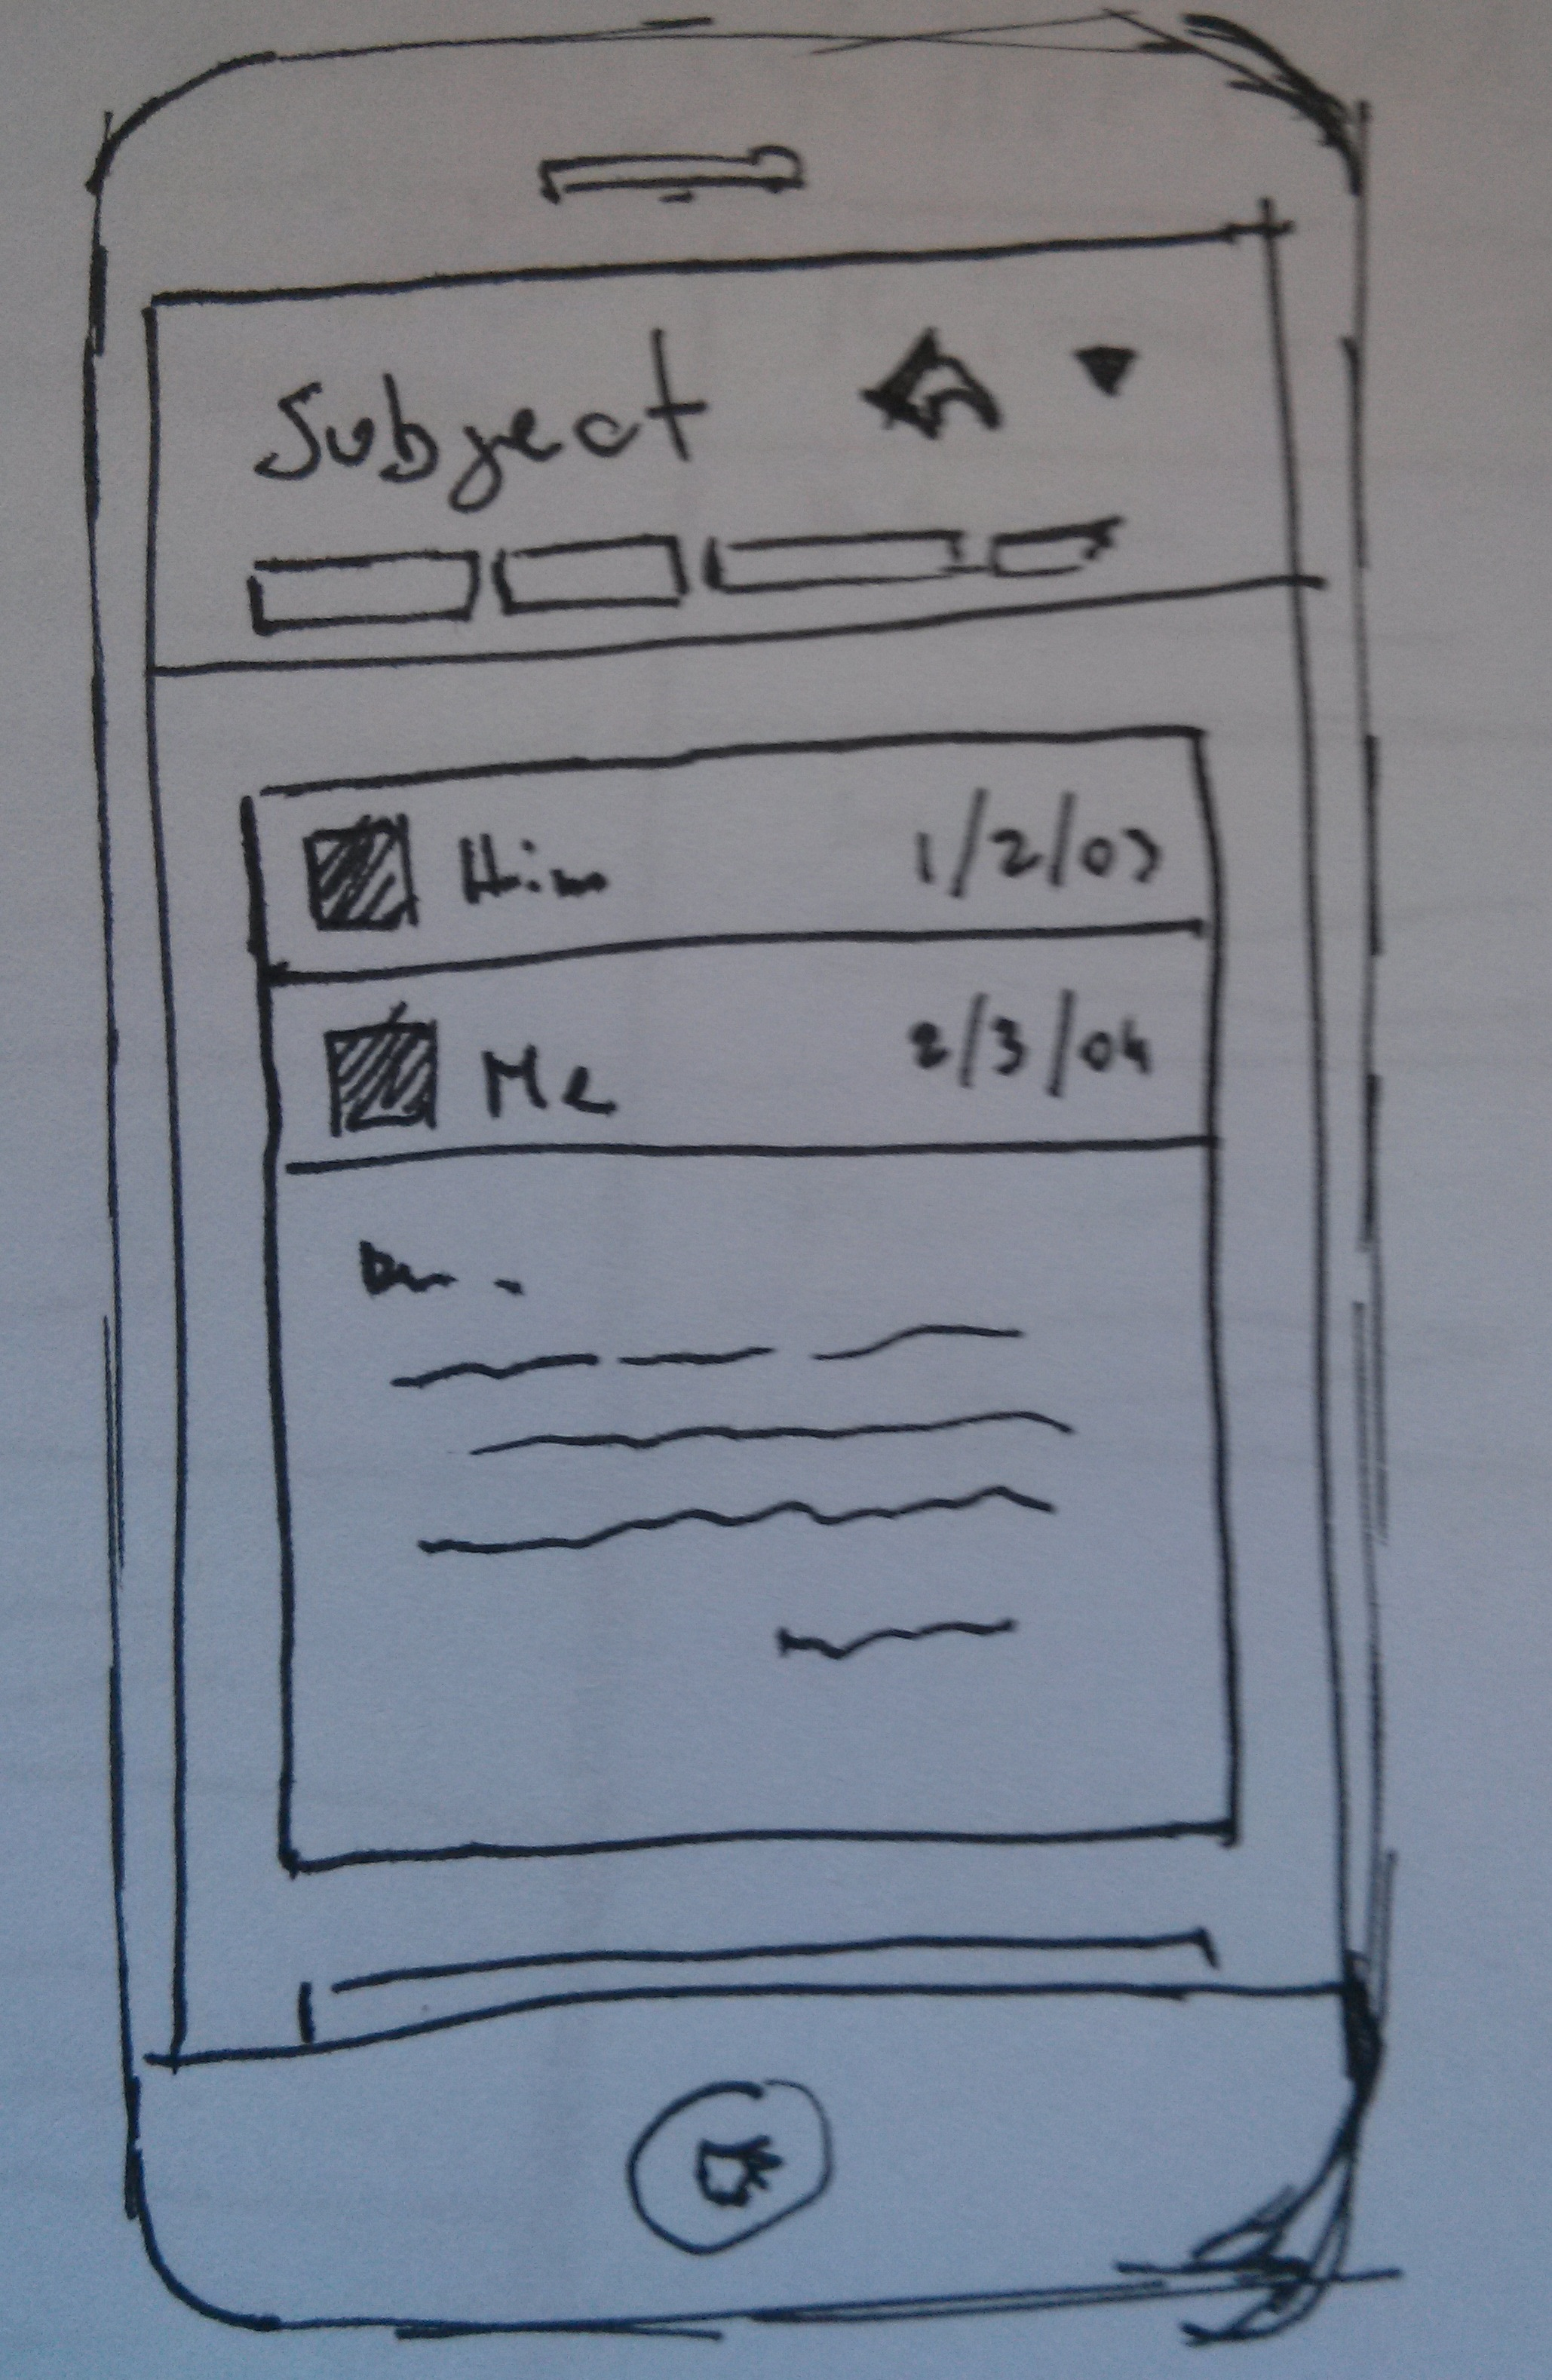
\includegraphics[height=2in]{email}
  \caption{the mobile version of \emph{bettermail}.}
  \label{fig:mobile}
\end{figure}
\subsection{Final result}

The steps presented in the previous section demonstrate the same step followed when designing and building the application. We present here some screenshots of the final result.

\begin{figure}[H]
  \centering
  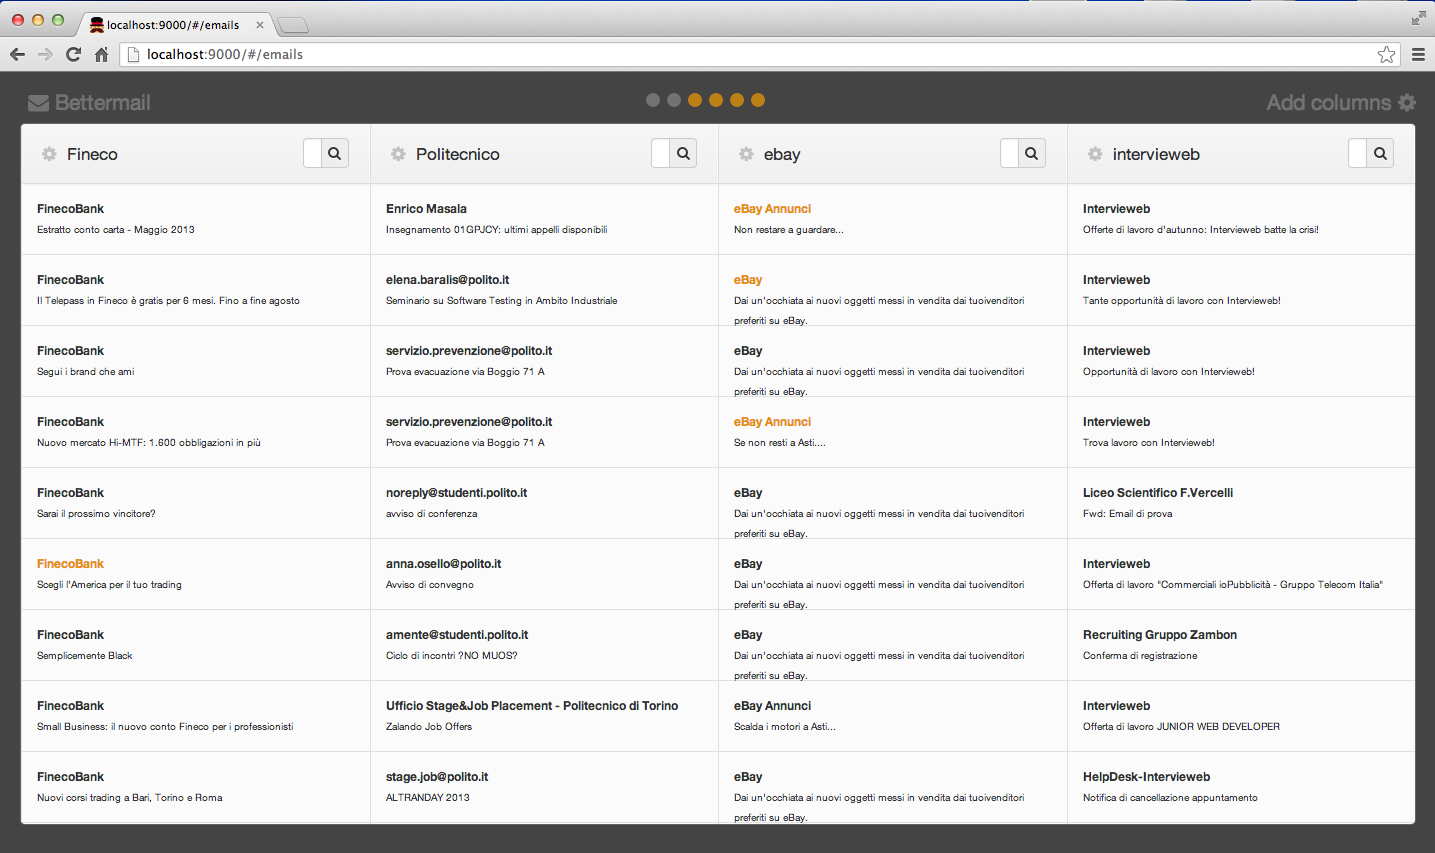
\includegraphics[width=4in]{main}
  \caption{The main interface of \emph{bettermail}.}
  \label{fig:main}
\end{figure}
In picture~\ref{fig:main} the main interface of the application is shown. It follows quite tightly the structure designed in the sketches, with a 4-column design, one per label, and a top bar for navigating between them.

\begin{figure}[H]
  \centering
  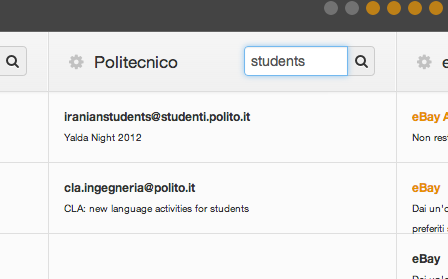
\includegraphics[width=4in]{main_search}
  \caption{\emph{bettermail} search capabilities,}
  \label{fig:main_search}
\end{figure}
Each column provides a collapsed search box which allow users to search for keyword in message subject and headers as shown in~\ref{fig:main_search}

\begin{figure}[H]
  \centering
  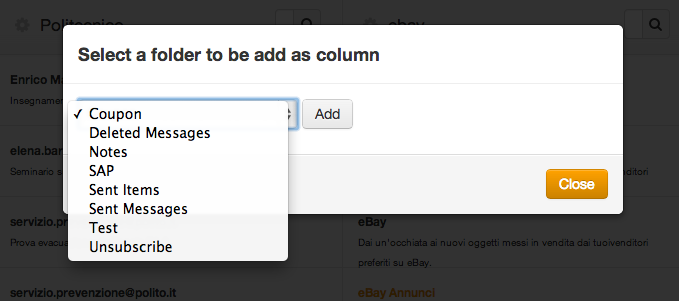
\includegraphics[width=4in]{main_modal_detail}
  
  \vspace{0.2in}

  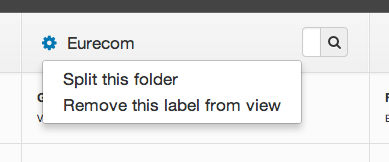
\includegraphics[width=4in]{main_options}
  \caption{The modal window for adding new columns and the drop-down menu for managing a column.}
  \label{fig:main_modal}
\end{figure}
Picture~\ref{fig:main_modal} shown two details of the applications: the modal box for adding new columns, accessible trough the top-right button and the drop-down option menu (one for each column) to remove it or access the clustering functionalities.

\begin{figure}[H]
  \centering
  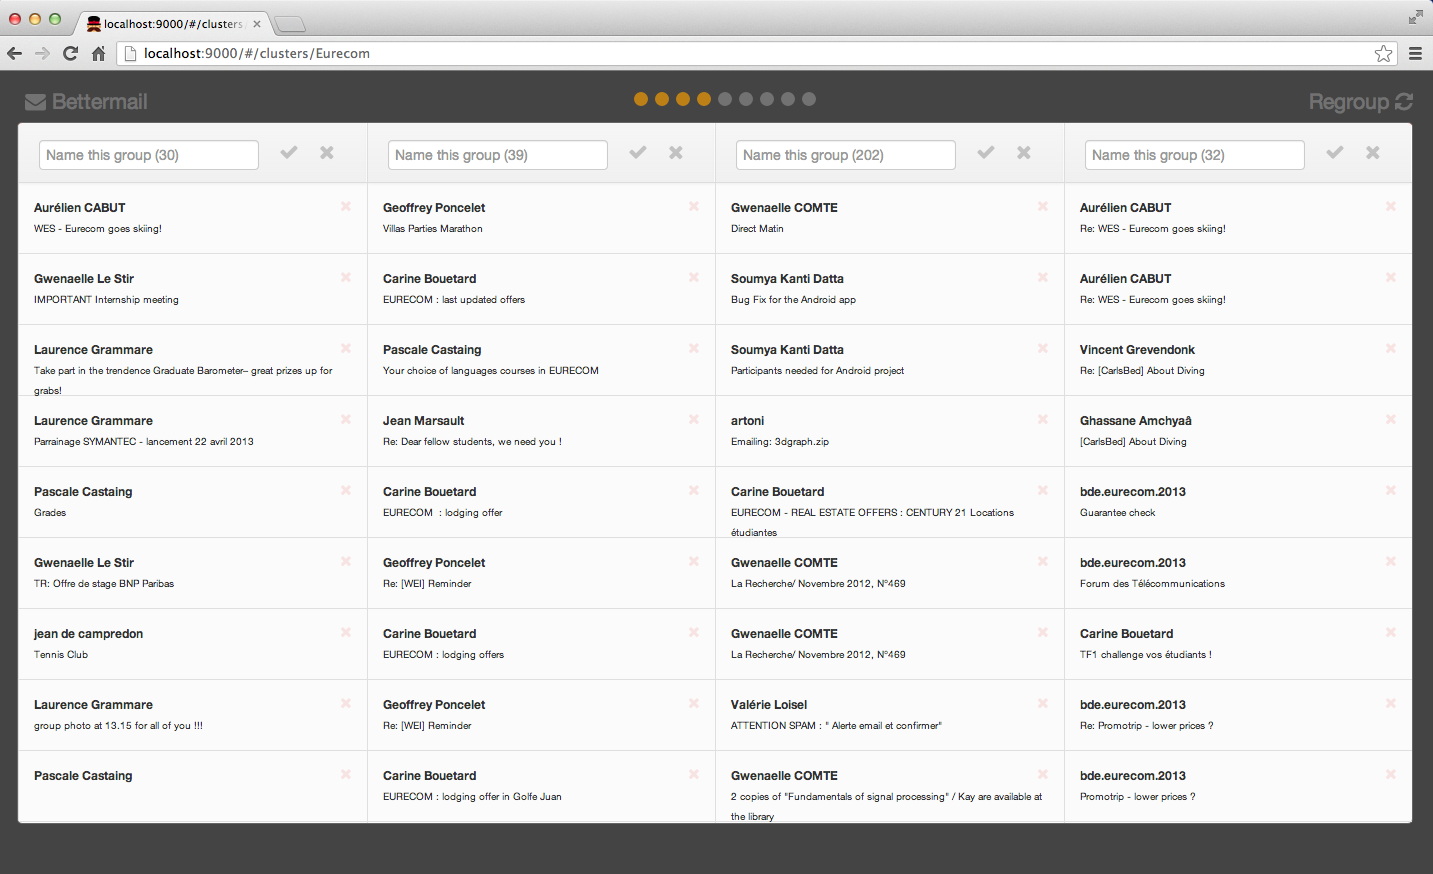
\includegraphics[width=4in]{clusters}
  
  \vspace{0.2in}

  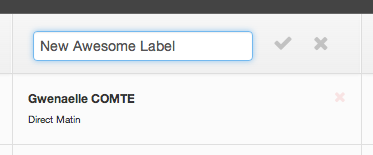
\includegraphics[width=3in]{clusters_detail}
  \caption{Main clustering window and the naming box detail.}
  \label{fig:cluster}
\end{figure}

We think that using the same pattern in both the main page and in that for cluster management is a plus both because it improves usability - the user already knew the interface - and because it fits well in the context: each column is a label subdivision and an overview of all this subdivision is easily accessed thanks to this kind of layout. The label name is replaced here by an input box for entering the new name and each cluster proposed can be accepted or declined individually.
Moreover, it is possible to instruct the system that a specific email does not belong to the specified cluster and thus remove it from the newly created box.

\section{Architecture}
As previously noted we decided to implement the client as a SPA. That is because interaction obtained thanks to the intensive use of XHR\footnote{the main object used for sending asynchronous HTTP requests.} it's widely considered ways better with respect to the classical multi-page model. In fact most web applications\footnote{the terms doesn't refer to general web sites but to complete applications built on top of the web platform like GMail, Cloud9IDE, Google Drive...} today prefer this model to offer a faster and more engaging UX to their customers. 

To better structure our work we use an MVC javascript framework chosen between Backbone.js, Ember and AngularJS. The first is the oldest and has many interesting feature, but it forces users to a specif type of data access, which is pretty far from plain javascript, and doesn't provide by itself a clear, structured way of developing the application. While Ember may be a good choice we choose the latter among these.
Because the choice of a framework strongly effects the overall architecture of the system, on the next section we will explain why we use AngularJS and how this choice effects the client structure.
\subsection{About AngularJS}
The reason behind our choice is to be found in the three main features of this framework, often denoted as \emph{3D} (Data Binding, Directives and Dependency Injection).
\subsubsection{Two ways data binding}
Most client-side frameworks offer some kind of templating system which allow to define how objects will be represented when attached to the DOM. These libraries offer a one-way data binding: if the object changes, the framework is notified and the DOM is altered accordingly.
AngularJS on the other end improves this approach in two ways: it uses plain HTML (even W3C compliant, if required) as the templating system and offers data binding in both directions: not only objects changes are reflected in the DOM, but the other way round too. If an input box is binded with a javascript variable, each time the input box is changed the variable itself is modified accordingly.
\subsubsection{Directives}
Front-end developers usually create or use widgets to encapsulate specific behavior in a single piece of code. Thanks to \emph{directives} it is possible to extend the native HTML markup language by \begin{quotation}
``teaching the browser new tricks''.
\begin{flushright}
Pavel Kozlowsky, Codemotion, Rome - 23 March 2013\footnote{http://www.youtube.com/watch?v=wmhPfx0s40o}
\end{flushright}
\end{quotation}
In other words it is possible to define your own tag and then use them like they were plain HTML; AngularJS compiles them in an internal representation and attaches the real HTML on the fly.
This feature provides two big advantages: you can build highly reusable components and the code looks much more cleaner and readable thanks to the extra markup being embedded in the directives. 
\subsubsection{Dependency Injection}
One of the main feature required by an industrial-ready system is to provide an easy way to unit test your components. AngularJS encourages developers to write separate modules; each module specifies the list of other modules it depends on, without explicitly allocating the resource itself (process handled by the framework). ``Requiring'' something instead of directly ``creating'' it make the components of an application much more decoupled (and thus, the whole easier to maintain). Moreover thanks to the ability to use different implementations of a specific component depending on the environment it becomes much easier to test this component independently: it is sufficient to provide a ``mocked'' version of a dependencies to avoid the need of having an instance of the real dependency up and running (this can be very useful if the dependency relies on some external service, it's slow or requires the system to change state, which is bad for unit testing).


As AngularJS is our framework of choice, the application follows the structure described by the framework itself:
\begin{itemize}
\item a set of \emph{service}s is responsible for creating an abstraction layer to access data. In our case we have services for retrieving data in the IndexedDB storage system of the browser (described later) and a service for accessing the REST API of our server.
\item a set of \emph{directive}s to encapsulate the behavior behind the graphical components of our applications 
\item some \emph{controller}s, responsible for binding data to the right HTML fragment (including event handlers).
\end{itemize}
\subsection{Tooling, scaffolding and external libraries}
In the last few years a lot of efforts have been put in improving and automating the workflow of front-end web development. A lot of tools and systems have been created in order to reduce developers efforts. 
Moreover, together with AngularJS we used other external resources to speed up and simplify the process. Here's a list of tools and external libraries of invaluable worth:
\begin{itemize}
\item Yeoman (yo - \texttt{http://yeoman.io}): a tool for project scaffolding. It creates a template web application including HTML5 boilerplate, EscmaScript 5 polyfill and many optionals libraries. Thanks to its excellent integration with AngularJS it can be invoked each time we need to create a new angular component (e.g to create a directive called \emph{tab}: \texttt{yo angular:directive tab}). Moreover it creates a complete and customized configuration file for \emph{Grunt}, described below
\item Grunt (\texttt{http://gruntjs.com}): used to build, preview and test the project, thanks to the help from tasks created using Yeoman it's very well integrated in the ecosystem. Specifically, it allows to run a static web server to serve file and try the systems, automatically compiles coffescript into javascript and SASS/SCSS into plain CSS every time a file changes, add support for in-browser livereload (again, on file changes). It integrates with Karma-runner, the javascript test runner developed by the AngularJS team. It allows to build the application by minifying and eventually optimizing javascript and CSS, compressing images and much more.
\item Bower (\texttt{http://bower.io}): it offers a solution to the front-end package management problem, as it allows to maintain and manage package installations and dependencies for generic front-end development resources (typically javascript and CSS libraries). 
\item Twitter Bootstrap (\texttt{http://twitter.github.io/bootstrap/}): a stylesheet framework which simplifies the development of user interfaces. It provides a grid system for layout definition and a wide set of components (buttons, tables, tooltips, etc...) 
\end{itemize}

\chapter{Evaluation}
\section{Clustering}
\subsection{Consideration on the personal dataset} % (fold)
\label{sub:consideration_on_the_personal_dataset}
The application has been developed with a strong focus on being working with real data. For that reason we choose our personal email account as the working dataset because we need the application to be able to operate on real IMAP connection. Therefore the definition and tuning for the clustering algorithm parameters has been done with subjective observation of the generated clusters.
The main problems found by this personal analysis are listed below: 
\begin{itemize}
  \item K-means generates some empty clusters (which are then ignored)
  \item Small and medium-size clusters are generally better than big ones
  \item False positives can be found even in small clusters.
  \item Very similar clusters are often disjointed 
\end{itemize}

Even if these consideration have very low scientific interest we find that are useful for better understanding how the clustering algorithm work on a dataset we know well. Moreover, having the whole application running on a real-life mailbox allows us to see it in action exactly like it would be in a production environment.

% subsection consideration_on_the_personal_dataset (end)

\subsection{Measures on ``enron'' dataset} % (fold)
\label{sub:measures_on_enron}
While a personal dataset may be good for personal evaluation and development it is good practice to test and measure performances on a well known dataset. Regarding email, the most widely used dataset available to the community is the ``Enron Corpus'', a large database of over 1.7 million emails generated by 158 employees of the Enron Corporation and now freely available without privacy and legal restrictions.
A lot of techniques exists for evaluate the goodness of a clustering algorithm. Because, for the time being, we only defined the distance functions while the algorithm itself is implemented by an external module, we will not use an internal evaluation criterion (intra-cluster and inter-cluster similarity) which requires knowledge of the cluster structure.
We suggest instead the use of normalized mutual information or NMI as an external evaluation criteria as described in \cite{Manning2008}.

% subsection measures_on_enron (end)

\section{Evaluation of the UX}
While designing and developing the application we tried to follow as much as possible a simple and coherent design, to get feedback from the project supervisors and from people around us to understand what should be done in order to improve it and make it better.
However, evaluating the user experience is generally a hard task, because it means investigating how a person feels about using a system which is subjective, context-dependent and dynamic over time.
A lot of different techniques have been developed both numerical (request people to fill in questionnaire and feedback form) and qualitative (Psychophysiological emotion measurements, Think aloud protocol, Expression observers) which requires people to be invited to a test and observed during this period.
Because we do not have neither a large user base nor the resources required for an emotion evaluation we will try a method based on two technique, both of them requiring a small community of users to be available.
\begin{itemize}
  \item Request users to give feedback and improvement advice on the github issue tracker (we suppose our community to be a small set of developer and enthusiast, used to this tool)
  \item Collect anonymous information on the application usage (time spent on each page, areas of the page clicked the most, feature usage), in order to better understand how people actually use the application.
\end{itemize}

\chapter{Conclusions and Future work}
We consider the first goal of this project reached: we give a proof of concept of how email managing can be innovated and adapted to users needs, both by providing new services and by new ideas in designing the user interface.

We feel that, while emails are an ``old'' technology, their use is so intense - especially for professionals - that it mustn't be underestimated. As previously described a lot of players are actively participating in exploring novel ideas in this field but it is not our interest to participate in this game as a competitor. 
On the other side we strongly believe in the open source community - from where the tool we used for building \emph{bettermail} mostly come from - and we would like to give something back to this world. Apart from the evaluation described in the previous chapter, we plan to improve this application in both the client and the server side in order for anyone to be able to deploy and use it, experiment and eventually improve it. For that reason all the source code both for the server and the client is publicly available on GitHub.\footnote{Respectively at https://github.com/artoale/betteremail-server and https://github.com/artoale/bettermail-client}

\section{On the client side}
\subsection{Mobile Web App} % (fold)
\label{sub:mobile_web_app}


The next step on the front end development is to make the adaptation required in order to enable this application to run on mobile devices. The concept (as you can see from the sketches) is already there, doesn't differ too much from the desktop version which is designed to be easily changed but some tweaking is still required in order to makes it work completely.
Moreover, because of the use of IndexedDB technology not available on Safari Mobile we need to add a shim\footnote{Shim: s small library that transparently intercepts an API and changes the parameters passed, handles the operation itself, or redirects the operation elsewhere - Wikipedia.} for it. IndexedDB over WebSQL\footnote{http://nparashuram.com/IndexedDBShim/} seems a reasonable choice because it would allow the application to work on both Safari, Chrome and Firefox mobile, giving the application a good browser support.
% subsection mobile_web_app (end)
\subsection{Full emailing feature} % (fold)
\label{sub:full_emailing_feature}
At this stage the application only support retrieval and classification of single email messages. Some important milestones in the future development of \emph{bettermail} are:
\begin{itemize}
  \item Client side support for emails thread (already supported by the backend)
  \item Attachment download
  \item Email reply implementation 
\end{itemize}

% subsection full_emailing_feature (end)
\section{On the server side}

Apart from the modification required in order to support the client side new feature we would like to experiment other solution, especially for the clustering algorithm. We plan to test Gibbs Latent Dirichlet Allocation - state of the art technique for free text clustering - against k-means. 
Moreover, before the application to be ready for production we need to implement security mechanism to allow authentication: we propose OpenID with OAuth as the main login pattern both because it is widely supported by many email providers and because it simplify the work of storing private authentication data.

\addcontentsline{toc}{chapter}{Bibliography}
\bibliography{biblio}

\appendix
\cleardoublepage
%\chapter{REVE ontology}
%\includegraphics[page=2,angle=-90, width=1.2\textwidth]{graphs.pdf}
%\chapter{Data model: focus on a person}
%\chapter{Data model: focus on a document}
%\chapter{Present state of the data}
%TODO : arranger l'orientation des pages pr l'impression ?

%\includepdf[pages=1-20]{fichier.pdf}
\end{document}
